\sectionthree{Insert, Delete, Find}
\begin{python0}
from solutions import *; clear()
\end{python0}

It's clear what you need to do for insert and find.
When you're given the key $k$, you hash to get $h(k)$.
If that's available, you put your key-value there.
If it's occupied, you probe using whatever method you have decided to use.
If your probe reaches the first hash value, you are in trouble.
At that point, you should probably throw an exception.

What about delete?
You might think that all you need to do is to find it
and then mark the row as available.
Hang on there ...

This means that you're breaking the chain of collided keys.
For instance if you're looking for a key that is hashed to
3 and there are four keys hashed to 3 and resolved using linear 
probes, then the three keys are at index values 3, 4, 5, 6.
If your key is at index 5, then marking that row as available,
when you search for the key at 6, your search algorithm is
going to stop at 5 and say it's not found. Duh.

There are several pretty obvious options.

\textsc{Option 1.}
Instead of a flag for each row saying
\textsc{Available}/\textsc{Not-Available},
you can have a flag that says
\textsc{Available}/\textsc{Not-Available}/\textsc{Deleted}.
In that case the available flag cannot (of course) cannot be a boolean.
During a search, if you see a row that is \textsc{Deleted},
you have to continue.
Your search ends if either you have found the key at a row that is
marked \textsc{Not-Available} or a row that is marked
\textsc{Available} or you reached
your first hash value.
Rows which are marked as \textsc{Deleted} are sometimes called tombstones.

The earlier table becomes:
\begin{center}
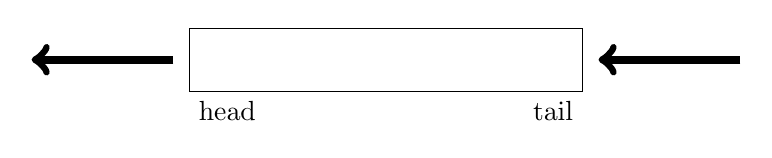
\begin{tikzpicture}

\draw (2.5, 0.4)
  node[draw, , , color=black,
       rounded corners=0cm, inner sep=0cm] {

\begin{minipage}[t][0.8cm]{5cm}
\mbox{}

\end{minipage}

};\draw[line width=0.1cm,black,->] (7,0.4) to  (5.2,0.4);
\draw[line width=0.1cm,black,->] (-0.2,0.4) to  (-2,0.4);

\node[anchor=north west] at (0,0)   {head};

\node[anchor=north east] at (5,0)   {tail};
\end{tikzpicture}

\end{center}



\textsc{Option 2.}
The second option is to organize the chain of collided keys by 
actually moving the keys to overwrite the row to be deleted.
For instance say your key is hashed to 3 and there four 
collided keys are index 3, 4, 5, 6.
Say your key is at index 4.
Then you have to move the data at index 5 to index 4 and index 6 to index 5
and then mark row 6 as available.
If there are not too many colliding keys and long probe sequences,
this is usually not that bad.
If the probe sequences are getting long, we will have to to a 
complete restructuring of the hash table -- see next section.

I will stick to \textsc{Option 1}.

Going back to out earlier table:
\begin{center}
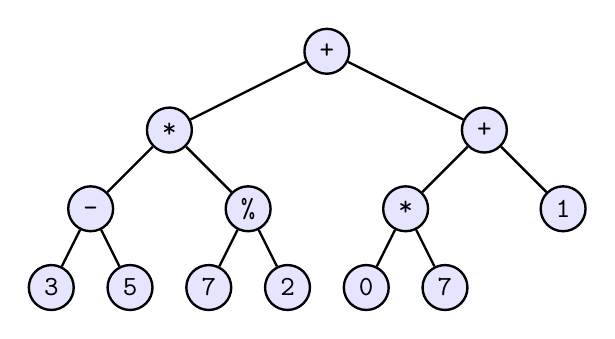
\begin{tikzpicture}

\fill[blue!10] (0.0, 0.0) circle (0.3);
\node [line width=0.03cm,black,minimum size=0.57cm,draw,circle] at (0.0,0.0)(+){};\draw (0.0, 0.0) node[color=black] {\texttt{+}};
\fill[blue!10] (-2.0, -1.0) circle (0.3);
\node [line width=0.03cm,black,minimum size=0.57cm,draw,circle] at (-2.0,-1.0)(*){};\draw (-2.0, -1.0) node[color=black] {\texttt{*}};
\fill[blue!10] (2.0, -1.0) circle (0.3);
\node [line width=0.03cm,black,minimum size=0.57cm,draw,circle] at (2.0,-1.0)(c){};\draw (2.0, -1.0) node[color=black] {\texttt{+}};
\fill[blue!10] (-3.0, -2.0) circle (0.3);
\node [line width=0.03cm,black,minimum size=0.57cm,draw,circle] at (-3.0,-2.0)(-){};\draw (-3.0, -2.0) node[color=black] {\texttt{-}};
\fill[blue!10] (-1.0, -2.0) circle (0.3);
\node [line width=0.03cm,black,minimum size=0.57cm,draw,circle] at (-1.0,-2.0)(e){};\draw (-1.0, -2.0) node[color=black] {\texttt{\%}};
\fill[blue!10] (1.0, -2.0) circle (0.3);
\node [line width=0.03cm,black,minimum size=0.57cm,draw,circle] at (1.0,-2.0)(f){};\draw (1.0, -2.0) node[color=black] {\texttt{*}};
\fill[blue!10] (3.0, -2.0) circle (0.3);
\node [line width=0.03cm,black,minimum size=0.57cm,draw,circle] at (3.0,-2.0)(1){};\draw (3.0, -2.0) node[color=black] {\texttt{1}};
\fill[blue!10] (-3.5, -3.0) circle (0.3);
\node [line width=0.03cm,black,minimum size=0.57cm,draw,circle] at (-3.5,-3.0)(3){};\draw (-3.5, -3.0) node[color=black] {\texttt{3}};
\fill[blue!10] (-2.5, -3.0) circle (0.3);
\node [line width=0.03cm,black,minimum size=0.57cm,draw,circle] at (-2.5,-3.0)(5){};\draw (-2.5, -3.0) node[color=black] {\texttt{5}};
\fill[blue!10] (-1.5, -3.0) circle (0.3);
\node [line width=0.03cm,black,minimum size=0.57cm,draw,circle] at (-1.5,-3.0)(z){};\draw (-1.5, -3.0) node[color=black] {\texttt{7}};
\fill[blue!10] (-0.5, -3.0) circle (0.3);
\node [line width=0.03cm,black,minimum size=0.57cm,draw,circle] at (-0.5,-3.0)(2){};\draw (-0.5, -3.0) node[color=black] {\texttt{2}};
\fill[blue!10] (0.5, -3.0) circle (0.3);
\node [line width=0.03cm,black,minimum size=0.57cm,draw,circle] at (0.5,-3.0)(0){};\draw (0.5, -3.0) node[color=black] {\texttt{0}};
\fill[blue!10] (1.5, -3.0) circle (0.3);
\node [line width=0.03cm,black,minimum size=0.57cm,draw,circle] at (1.5,-3.0)(7){};\draw (1.5, -3.0) node[color=black] {\texttt{7}};\draw[line width=0.03cm,black] (+) to  (*);
\draw[line width=0.03cm,black] (+) to  (c);
\draw[line width=0.03cm,black] (*) to  (-);
\draw[line width=0.03cm,black] (*) to  (e);
\draw[line width=0.03cm,black] (c) to  (f);
\draw[line width=0.03cm,black] (c) to  (1);
\draw[line width=0.03cm,black] (-) to  (3);
\draw[line width=0.03cm,black] (-) to  (5);
\draw[line width=0.03cm,black] (e) to  (z);
\draw[line width=0.03cm,black] (e) to  (2);
\draw[line width=0.03cm,black] (f) to  (0);
\draw[line width=0.03cm,black] (f) to  (7);
\end{tikzpicture}

\end{center}



If I add 
\texttt{(Tammy, 6.2)}
and
then 
\texttt{(Andrew, 5.7)}.
and
then 
\texttt{(Tania, 6.7)},
this is the resulting table:

\begin{center}
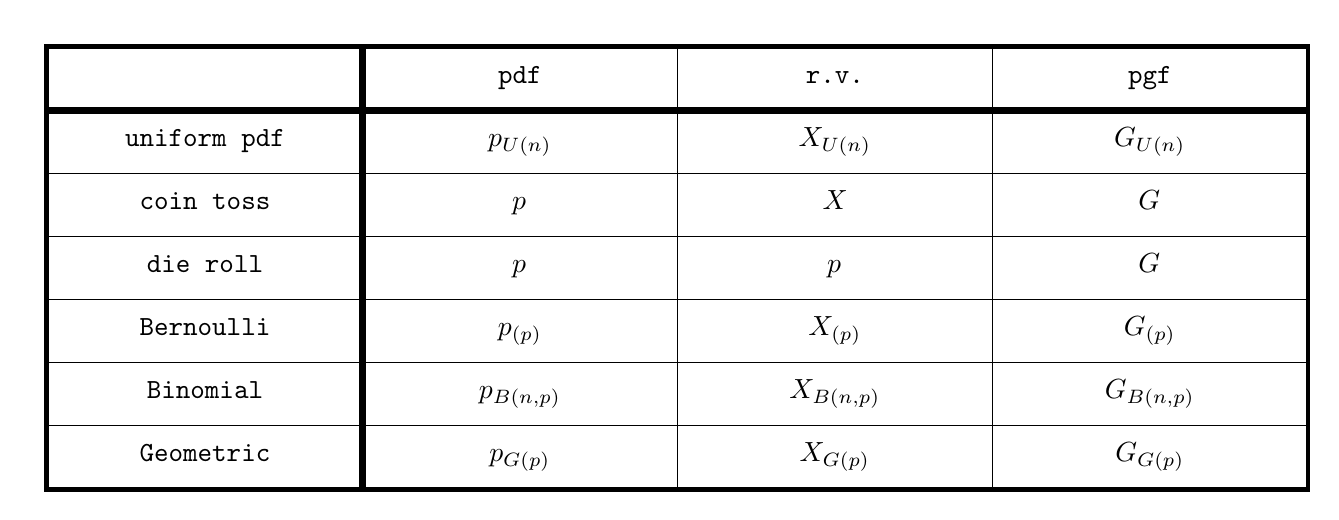
\begin{tikzpicture}

\draw (2.0, -0.4)
  node[draw, line width=0.02cm, , color=black,
       rounded corners=0cm, inner sep=0cm] {

\begin{minipage}[t][0.8cm]{4.0cm}
\mbox{}

\end{minipage}

};\draw (2.0, -0.4) node[color=black] {{\texttt{{\vphantom{pdfr.v.pgfuniform pdfcoin tossdie rollBernoulliBinomialGeometric$p_{U(n)}$$X_{U(n)}$$G_{U(n)}$$p_{\COIN}$$X_{\COIN}$$G_{\COIN}$$p_{\DIE}$$G_{\DIE}$$p_{\BERNOULLI(p)}$$X_{\BERNOULLI(p)}$$G_{\BERNOULLI(p)}$$p_{B(n,p)}$$X_{B(n,p)}$$G_{B(n,p)}$$p_{G(p)}$$X_{G(p)}$$G_{G(p)}$}}}}};\node[anchor=south] at (2.0,0.01) {};\node[anchor=east] at (-0.01,-0.4) {};
\draw (2.0, -0.4)
  node[draw, line width=0.06cm, , color=black,
       rounded corners=0cm, inner sep=0cm] {

\begin{minipage}[t][0.82cm]{4.02cm}
\mbox{}

\end{minipage}

};
\draw (6.0, -0.4)
  node[draw, line width=0.02cm, , color=black,
       rounded corners=0cm, inner sep=0cm] {

\begin{minipage}[t][0.8cm]{4.0cm}
\mbox{}

\end{minipage}

};\draw (6.0, -0.4) node[color=black] {{\texttt{{\vphantom{pdfr.v.pgfuniform pdfcoin tossdie rollBernoulliBinomialGeometric$p_{U(n)}$$X_{U(n)}$$G_{U(n)}$$p_{\COIN}$$X_{\COIN}$$G_{\COIN}$$p_{\DIE}$$G_{\DIE}$$p_{\BERNOULLI(p)}$$X_{\BERNOULLI(p)}$$G_{\BERNOULLI(p)}$$p_{B(n,p)}$$X_{B(n,p)}$$G_{B(n,p)}$$p_{G(p)}$$X_{G(p)}$$G_{G(p)}$}pdf}}}};
\draw (10.0, -0.4)
  node[draw, line width=0.02cm, , color=black,
       rounded corners=0cm, inner sep=0cm] {

\begin{minipage}[t][0.8cm]{4.0cm}
\mbox{}

\end{minipage}

};\draw (10.0, -0.4) node[color=black] {{\texttt{{\vphantom{pdfr.v.pgfuniform pdfcoin tossdie rollBernoulliBinomialGeometric$p_{U(n)}$$X_{U(n)}$$G_{U(n)}$$p_{\COIN}$$X_{\COIN}$$G_{\COIN}$$p_{\DIE}$$G_{\DIE}$$p_{\BERNOULLI(p)}$$X_{\BERNOULLI(p)}$$G_{\BERNOULLI(p)}$$p_{B(n,p)}$$X_{B(n,p)}$$G_{B(n,p)}$$p_{G(p)}$$X_{G(p)}$$G_{G(p)}$}r.v.}}}};
\draw (14.0, -0.4)
  node[draw, line width=0.02cm, , color=black,
       rounded corners=0cm, inner sep=0cm] {

\begin{minipage}[t][0.8cm]{4.0cm}
\mbox{}

\end{minipage}

};\draw (14.0, -0.4) node[color=black] {{\texttt{{\vphantom{pdfr.v.pgfuniform pdfcoin tossdie rollBernoulliBinomialGeometric$p_{U(n)}$$X_{U(n)}$$G_{U(n)}$$p_{\COIN}$$X_{\COIN}$$G_{\COIN}$$p_{\DIE}$$G_{\DIE}$$p_{\BERNOULLI(p)}$$X_{\BERNOULLI(p)}$$G_{\BERNOULLI(p)}$$p_{B(n,p)}$$X_{B(n,p)}$$G_{B(n,p)}$$p_{G(p)}$$X_{G(p)}$$G_{G(p)}$}pgf}}}};\node[anchor=south] at (6.0,0.01) {};\node[anchor=south] at (10.0,0.01) {};\node[anchor=south] at (14.0,0.01) {};\node[anchor=east] at (3.99,-0.4) {};
\draw (10.000000000000002, -0.4)
  node[draw, line width=0.06cm, , color=black,
       rounded corners=0cm, inner sep=0cm] {

\begin{minipage}[t][0.82cm]{12.02cm}
\mbox{}

\end{minipage}

};
\draw (2.0, -1.2000000000000002)
  node[draw, line width=0.02cm, , color=black,
       rounded corners=0cm, inner sep=0cm] {

\begin{minipage}[t][0.8cm]{4.0cm}
\mbox{}

\end{minipage}

};\draw (2.0, -1.2000000000000002) node[color=black] {{\texttt{{\vphantom{pdfr.v.pgfuniform pdfcoin tossdie rollBernoulliBinomialGeometric$p_{U(n)}$$X_{U(n)}$$G_{U(n)}$$p_{\COIN}$$X_{\COIN}$$G_{\COIN}$$p_{\DIE}$$G_{\DIE}$$p_{\BERNOULLI(p)}$$X_{\BERNOULLI(p)}$$G_{\BERNOULLI(p)}$$p_{B(n,p)}$$X_{B(n,p)}$$G_{B(n,p)}$$p_{G(p)}$$X_{G(p)}$$G_{G(p)}$}uniform pdf}}}};
\draw (2.0, -2.0)
  node[draw, line width=0.02cm, , color=black,
       rounded corners=0cm, inner sep=0cm] {

\begin{minipage}[t][0.8cm]{4.0cm}
\mbox{}

\end{minipage}

};\draw (2.0, -2.0) node[color=black] {{\texttt{{\vphantom{pdfr.v.pgfuniform pdfcoin tossdie rollBernoulliBinomialGeometric$p_{U(n)}$$X_{U(n)}$$G_{U(n)}$$p_{\COIN}$$X_{\COIN}$$G_{\COIN}$$p_{\DIE}$$G_{\DIE}$$p_{\BERNOULLI(p)}$$X_{\BERNOULLI(p)}$$G_{\BERNOULLI(p)}$$p_{B(n,p)}$$X_{B(n,p)}$$G_{B(n,p)}$$p_{G(p)}$$X_{G(p)}$$G_{G(p)}$}coin toss}}}};
\draw (2.0, -2.8000000000000003)
  node[draw, line width=0.02cm, , color=black,
       rounded corners=0cm, inner sep=0cm] {

\begin{minipage}[t][0.8cm]{4.0cm}
\mbox{}

\end{minipage}

};\draw (2.0, -2.8000000000000003) node[color=black] {{\texttt{{\vphantom{pdfr.v.pgfuniform pdfcoin tossdie rollBernoulliBinomialGeometric$p_{U(n)}$$X_{U(n)}$$G_{U(n)}$$p_{\COIN}$$X_{\COIN}$$G_{\COIN}$$p_{\DIE}$$G_{\DIE}$$p_{\BERNOULLI(p)}$$X_{\BERNOULLI(p)}$$G_{\BERNOULLI(p)}$$p_{B(n,p)}$$X_{B(n,p)}$$G_{B(n,p)}$$p_{G(p)}$$X_{G(p)}$$G_{G(p)}$}die roll}}}};
\draw (2.0, -3.6)
  node[draw, line width=0.02cm, , color=black,
       rounded corners=0cm, inner sep=0cm] {

\begin{minipage}[t][0.8cm]{4.0cm}
\mbox{}

\end{minipage}

};\draw (2.0, -3.6) node[color=black] {{\texttt{{\vphantom{pdfr.v.pgfuniform pdfcoin tossdie rollBernoulliBinomialGeometric$p_{U(n)}$$X_{U(n)}$$G_{U(n)}$$p_{\COIN}$$X_{\COIN}$$G_{\COIN}$$p_{\DIE}$$G_{\DIE}$$p_{\BERNOULLI(p)}$$X_{\BERNOULLI(p)}$$G_{\BERNOULLI(p)}$$p_{B(n,p)}$$X_{B(n,p)}$$G_{B(n,p)}$$p_{G(p)}$$X_{G(p)}$$G_{G(p)}$}Bernoulli}}}};
\draw (2.0, -4.4)
  node[draw, line width=0.02cm, , color=black,
       rounded corners=0cm, inner sep=0cm] {

\begin{minipage}[t][0.8cm]{4.0cm}
\mbox{}

\end{minipage}

};\draw (2.0, -4.4) node[color=black] {{\texttt{{\vphantom{pdfr.v.pgfuniform pdfcoin tossdie rollBernoulliBinomialGeometric$p_{U(n)}$$X_{U(n)}$$G_{U(n)}$$p_{\COIN}$$X_{\COIN}$$G_{\COIN}$$p_{\DIE}$$G_{\DIE}$$p_{\BERNOULLI(p)}$$X_{\BERNOULLI(p)}$$G_{\BERNOULLI(p)}$$p_{B(n,p)}$$X_{B(n,p)}$$G_{B(n,p)}$$p_{G(p)}$$X_{G(p)}$$G_{G(p)}$}Binomial}}}};
\draw (2.0, -5.199999999999999)
  node[draw, line width=0.02cm, , color=black,
       rounded corners=0cm, inner sep=0cm] {

\begin{minipage}[t][0.8cm]{4.0cm}
\mbox{}

\end{minipage}

};\draw (2.0, -5.199999999999999) node[color=black] {{\texttt{{\vphantom{pdfr.v.pgfuniform pdfcoin tossdie rollBernoulliBinomialGeometric$p_{U(n)}$$X_{U(n)}$$G_{U(n)}$$p_{\COIN}$$X_{\COIN}$$G_{\COIN}$$p_{\DIE}$$G_{\DIE}$$p_{\BERNOULLI(p)}$$X_{\BERNOULLI(p)}$$G_{\BERNOULLI(p)}$$p_{B(n,p)}$$X_{B(n,p)}$$G_{B(n,p)}$$p_{G(p)}$$X_{G(p)}$$G_{G(p)}$}Geometric}}}};\node[anchor=south] at (2.0,-0.79) {};\node[anchor=east] at (-0.01,-1.2000000000000002) {};\node[anchor=east] at (-0.01,-2.0000000000000004) {};\node[anchor=east] at (-0.01,-2.8000000000000003) {};\node[anchor=east] at (-0.01,-3.6) {};\node[anchor=east] at (-0.01,-4.4) {};\node[anchor=east] at (-0.01,-5.199999999999999) {};
\draw (2.0, -3.1999999999999997)
  node[draw, line width=0.06cm, , color=black,
       rounded corners=0cm, inner sep=0cm] {

\begin{minipage}[t][4.82cm]{4.02cm}
\mbox{}

\end{minipage}

};
\draw (6.0, -1.2000000000000002)
  node[draw, line width=0.02cm, , color=black,
       rounded corners=0cm, inner sep=0cm] {

\begin{minipage}[t][0.8cm]{4.0cm}
\mbox{}

\end{minipage}

};\draw (6.0, -1.2000000000000002) node[color=black] {{\texttt{{\vphantom{pdfr.v.pgfuniform pdfcoin tossdie rollBernoulliBinomialGeometric$p_{U(n)}$$X_{U(n)}$$G_{U(n)}$$p_{\COIN}$$X_{\COIN}$$G_{\COIN}$$p_{\DIE}$$G_{\DIE}$$p_{\BERNOULLI(p)}$$X_{\BERNOULLI(p)}$$G_{\BERNOULLI(p)}$$p_{B(n,p)}$$X_{B(n,p)}$$G_{B(n,p)}$$p_{G(p)}$$X_{G(p)}$$G_{G(p)}$}$p_{U(n)}$}}}};
\draw (10.0, -1.2000000000000002)
  node[draw, line width=0.02cm, , color=black,
       rounded corners=0cm, inner sep=0cm] {

\begin{minipage}[t][0.8cm]{4.0cm}
\mbox{}

\end{minipage}

};\draw (10.0, -1.2000000000000002) node[color=black] {{\texttt{{\vphantom{pdfr.v.pgfuniform pdfcoin tossdie rollBernoulliBinomialGeometric$p_{U(n)}$$X_{U(n)}$$G_{U(n)}$$p_{\COIN}$$X_{\COIN}$$G_{\COIN}$$p_{\DIE}$$G_{\DIE}$$p_{\BERNOULLI(p)}$$X_{\BERNOULLI(p)}$$G_{\BERNOULLI(p)}$$p_{B(n,p)}$$X_{B(n,p)}$$G_{B(n,p)}$$p_{G(p)}$$X_{G(p)}$$G_{G(p)}$}$X_{U(n)}$}}}};
\draw (14.0, -1.2000000000000002)
  node[draw, line width=0.02cm, , color=black,
       rounded corners=0cm, inner sep=0cm] {

\begin{minipage}[t][0.8cm]{4.0cm}
\mbox{}

\end{minipage}

};\draw (14.0, -1.2000000000000002) node[color=black] {{\texttt{{\vphantom{pdfr.v.pgfuniform pdfcoin tossdie rollBernoulliBinomialGeometric$p_{U(n)}$$X_{U(n)}$$G_{U(n)}$$p_{\COIN}$$X_{\COIN}$$G_{\COIN}$$p_{\DIE}$$G_{\DIE}$$p_{\BERNOULLI(p)}$$X_{\BERNOULLI(p)}$$G_{\BERNOULLI(p)}$$p_{B(n,p)}$$X_{B(n,p)}$$G_{B(n,p)}$$p_{G(p)}$$X_{G(p)}$$G_{G(p)}$}$G_{U(n)}$}}}};
\draw (6.0, -2.0)
  node[draw, line width=0.02cm, , color=black,
       rounded corners=0cm, inner sep=0cm] {

\begin{minipage}[t][0.8cm]{4.0cm}
\mbox{}

\end{minipage}

};\draw (6.0, -2.0) node[color=black] {{\texttt{{\vphantom{pdfr.v.pgfuniform pdfcoin tossdie rollBernoulliBinomialGeometric$p_{U(n)}$$X_{U(n)}$$G_{U(n)}$$p_{\COIN}$$X_{\COIN}$$G_{\COIN}$$p_{\DIE}$$G_{\DIE}$$p_{\BERNOULLI(p)}$$X_{\BERNOULLI(p)}$$G_{\BERNOULLI(p)}$$p_{B(n,p)}$$X_{B(n,p)}$$G_{B(n,p)}$$p_{G(p)}$$X_{G(p)}$$G_{G(p)}$}$p_{\COIN}$}}}};
\draw (10.0, -2.0)
  node[draw, line width=0.02cm, , color=black,
       rounded corners=0cm, inner sep=0cm] {

\begin{minipage}[t][0.8cm]{4.0cm}
\mbox{}

\end{minipage}

};\draw (10.0, -2.0) node[color=black] {{\texttt{{\vphantom{pdfr.v.pgfuniform pdfcoin tossdie rollBernoulliBinomialGeometric$p_{U(n)}$$X_{U(n)}$$G_{U(n)}$$p_{\COIN}$$X_{\COIN}$$G_{\COIN}$$p_{\DIE}$$G_{\DIE}$$p_{\BERNOULLI(p)}$$X_{\BERNOULLI(p)}$$G_{\BERNOULLI(p)}$$p_{B(n,p)}$$X_{B(n,p)}$$G_{B(n,p)}$$p_{G(p)}$$X_{G(p)}$$G_{G(p)}$}$X_{\COIN}$}}}};
\draw (14.0, -2.0)
  node[draw, line width=0.02cm, , color=black,
       rounded corners=0cm, inner sep=0cm] {

\begin{minipage}[t][0.8cm]{4.0cm}
\mbox{}

\end{minipage}

};\draw (14.0, -2.0) node[color=black] {{\texttt{{\vphantom{pdfr.v.pgfuniform pdfcoin tossdie rollBernoulliBinomialGeometric$p_{U(n)}$$X_{U(n)}$$G_{U(n)}$$p_{\COIN}$$X_{\COIN}$$G_{\COIN}$$p_{\DIE}$$G_{\DIE}$$p_{\BERNOULLI(p)}$$X_{\BERNOULLI(p)}$$G_{\BERNOULLI(p)}$$p_{B(n,p)}$$X_{B(n,p)}$$G_{B(n,p)}$$p_{G(p)}$$X_{G(p)}$$G_{G(p)}$}$G_{\COIN}$}}}};
\draw (6.0, -2.8000000000000003)
  node[draw, line width=0.02cm, , color=black,
       rounded corners=0cm, inner sep=0cm] {

\begin{minipage}[t][0.8cm]{4.0cm}
\mbox{}

\end{minipage}

};\draw (6.0, -2.8000000000000003) node[color=black] {{\texttt{{\vphantom{pdfr.v.pgfuniform pdfcoin tossdie rollBernoulliBinomialGeometric$p_{U(n)}$$X_{U(n)}$$G_{U(n)}$$p_{\COIN}$$X_{\COIN}$$G_{\COIN}$$p_{\DIE}$$G_{\DIE}$$p_{\BERNOULLI(p)}$$X_{\BERNOULLI(p)}$$G_{\BERNOULLI(p)}$$p_{B(n,p)}$$X_{B(n,p)}$$G_{B(n,p)}$$p_{G(p)}$$X_{G(p)}$$G_{G(p)}$}$p_{\DIE}$}}}};
\draw (10.0, -2.8000000000000003)
  node[draw, line width=0.02cm, , color=black,
       rounded corners=0cm, inner sep=0cm] {

\begin{minipage}[t][0.8cm]{4.0cm}
\mbox{}

\end{minipage}

};\draw (10.0, -2.8000000000000003) node[color=black] {{\texttt{{\vphantom{pdfr.v.pgfuniform pdfcoin tossdie rollBernoulliBinomialGeometric$p_{U(n)}$$X_{U(n)}$$G_{U(n)}$$p_{\COIN}$$X_{\COIN}$$G_{\COIN}$$p_{\DIE}$$G_{\DIE}$$p_{\BERNOULLI(p)}$$X_{\BERNOULLI(p)}$$G_{\BERNOULLI(p)}$$p_{B(n,p)}$$X_{B(n,p)}$$G_{B(n,p)}$$p_{G(p)}$$X_{G(p)}$$G_{G(p)}$}$p_{\DIE}$}}}};
\draw (14.0, -2.8000000000000003)
  node[draw, line width=0.02cm, , color=black,
       rounded corners=0cm, inner sep=0cm] {

\begin{minipage}[t][0.8cm]{4.0cm}
\mbox{}

\end{minipage}

};\draw (14.0, -2.8000000000000003) node[color=black] {{\texttt{{\vphantom{pdfr.v.pgfuniform pdfcoin tossdie rollBernoulliBinomialGeometric$p_{U(n)}$$X_{U(n)}$$G_{U(n)}$$p_{\COIN}$$X_{\COIN}$$G_{\COIN}$$p_{\DIE}$$G_{\DIE}$$p_{\BERNOULLI(p)}$$X_{\BERNOULLI(p)}$$G_{\BERNOULLI(p)}$$p_{B(n,p)}$$X_{B(n,p)}$$G_{B(n,p)}$$p_{G(p)}$$X_{G(p)}$$G_{G(p)}$}$G_{\DIE}$}}}};
\draw (6.0, -3.6)
  node[draw, line width=0.02cm, , color=black,
       rounded corners=0cm, inner sep=0cm] {

\begin{minipage}[t][0.8cm]{4.0cm}
\mbox{}

\end{minipage}

};\draw (6.0, -3.6) node[color=black] {{\texttt{{\vphantom{pdfr.v.pgfuniform pdfcoin tossdie rollBernoulliBinomialGeometric$p_{U(n)}$$X_{U(n)}$$G_{U(n)}$$p_{\COIN}$$X_{\COIN}$$G_{\COIN}$$p_{\DIE}$$G_{\DIE}$$p_{\BERNOULLI(p)}$$X_{\BERNOULLI(p)}$$G_{\BERNOULLI(p)}$$p_{B(n,p)}$$X_{B(n,p)}$$G_{B(n,p)}$$p_{G(p)}$$X_{G(p)}$$G_{G(p)}$}$p_{\BERNOULLI(p)}$}}}};
\draw (10.0, -3.6)
  node[draw, line width=0.02cm, , color=black,
       rounded corners=0cm, inner sep=0cm] {

\begin{minipage}[t][0.8cm]{4.0cm}
\mbox{}

\end{minipage}

};\draw (10.0, -3.6) node[color=black] {{\texttt{{\vphantom{pdfr.v.pgfuniform pdfcoin tossdie rollBernoulliBinomialGeometric$p_{U(n)}$$X_{U(n)}$$G_{U(n)}$$p_{\COIN}$$X_{\COIN}$$G_{\COIN}$$p_{\DIE}$$G_{\DIE}$$p_{\BERNOULLI(p)}$$X_{\BERNOULLI(p)}$$G_{\BERNOULLI(p)}$$p_{B(n,p)}$$X_{B(n,p)}$$G_{B(n,p)}$$p_{G(p)}$$X_{G(p)}$$G_{G(p)}$}$X_{\BERNOULLI(p)}$}}}};
\draw (14.0, -3.6)
  node[draw, line width=0.02cm, , color=black,
       rounded corners=0cm, inner sep=0cm] {

\begin{minipage}[t][0.8cm]{4.0cm}
\mbox{}

\end{minipage}

};\draw (14.0, -3.6) node[color=black] {{\texttt{{\vphantom{pdfr.v.pgfuniform pdfcoin tossdie rollBernoulliBinomialGeometric$p_{U(n)}$$X_{U(n)}$$G_{U(n)}$$p_{\COIN}$$X_{\COIN}$$G_{\COIN}$$p_{\DIE}$$G_{\DIE}$$p_{\BERNOULLI(p)}$$X_{\BERNOULLI(p)}$$G_{\BERNOULLI(p)}$$p_{B(n,p)}$$X_{B(n,p)}$$G_{B(n,p)}$$p_{G(p)}$$X_{G(p)}$$G_{G(p)}$}$G_{\BERNOULLI(p)}$}}}};
\draw (6.0, -4.4)
  node[draw, line width=0.02cm, , color=black,
       rounded corners=0cm, inner sep=0cm] {

\begin{minipage}[t][0.8cm]{4.0cm}
\mbox{}

\end{minipage}

};\draw (6.0, -4.4) node[color=black] {{\texttt{{\vphantom{pdfr.v.pgfuniform pdfcoin tossdie rollBernoulliBinomialGeometric$p_{U(n)}$$X_{U(n)}$$G_{U(n)}$$p_{\COIN}$$X_{\COIN}$$G_{\COIN}$$p_{\DIE}$$G_{\DIE}$$p_{\BERNOULLI(p)}$$X_{\BERNOULLI(p)}$$G_{\BERNOULLI(p)}$$p_{B(n,p)}$$X_{B(n,p)}$$G_{B(n,p)}$$p_{G(p)}$$X_{G(p)}$$G_{G(p)}$}$p_{B(n,p)}$}}}};
\draw (10.0, -4.4)
  node[draw, line width=0.02cm, , color=black,
       rounded corners=0cm, inner sep=0cm] {

\begin{minipage}[t][0.8cm]{4.0cm}
\mbox{}

\end{minipage}

};\draw (10.0, -4.4) node[color=black] {{\texttt{{\vphantom{pdfr.v.pgfuniform pdfcoin tossdie rollBernoulliBinomialGeometric$p_{U(n)}$$X_{U(n)}$$G_{U(n)}$$p_{\COIN}$$X_{\COIN}$$G_{\COIN}$$p_{\DIE}$$G_{\DIE}$$p_{\BERNOULLI(p)}$$X_{\BERNOULLI(p)}$$G_{\BERNOULLI(p)}$$p_{B(n,p)}$$X_{B(n,p)}$$G_{B(n,p)}$$p_{G(p)}$$X_{G(p)}$$G_{G(p)}$}$X_{B(n,p)}$}}}};
\draw (14.0, -4.4)
  node[draw, line width=0.02cm, , color=black,
       rounded corners=0cm, inner sep=0cm] {

\begin{minipage}[t][0.8cm]{4.0cm}
\mbox{}

\end{minipage}

};\draw (14.0, -4.4) node[color=black] {{\texttt{{\vphantom{pdfr.v.pgfuniform pdfcoin tossdie rollBernoulliBinomialGeometric$p_{U(n)}$$X_{U(n)}$$G_{U(n)}$$p_{\COIN}$$X_{\COIN}$$G_{\COIN}$$p_{\DIE}$$G_{\DIE}$$p_{\BERNOULLI(p)}$$X_{\BERNOULLI(p)}$$G_{\BERNOULLI(p)}$$p_{B(n,p)}$$X_{B(n,p)}$$G_{B(n,p)}$$p_{G(p)}$$X_{G(p)}$$G_{G(p)}$}$G_{B(n,p)}$}}}};
\draw (6.0, -5.199999999999999)
  node[draw, line width=0.02cm, , color=black,
       rounded corners=0cm, inner sep=0cm] {

\begin{minipage}[t][0.8cm]{4.0cm}
\mbox{}

\end{minipage}

};\draw (6.0, -5.199999999999999) node[color=black] {{\texttt{{\vphantom{pdfr.v.pgfuniform pdfcoin tossdie rollBernoulliBinomialGeometric$p_{U(n)}$$X_{U(n)}$$G_{U(n)}$$p_{\COIN}$$X_{\COIN}$$G_{\COIN}$$p_{\DIE}$$G_{\DIE}$$p_{\BERNOULLI(p)}$$X_{\BERNOULLI(p)}$$G_{\BERNOULLI(p)}$$p_{B(n,p)}$$X_{B(n,p)}$$G_{B(n,p)}$$p_{G(p)}$$X_{G(p)}$$G_{G(p)}$}$p_{G(p)}$}}}};
\draw (10.0, -5.199999999999999)
  node[draw, line width=0.02cm, , color=black,
       rounded corners=0cm, inner sep=0cm] {

\begin{minipage}[t][0.8cm]{4.0cm}
\mbox{}

\end{minipage}

};\draw (10.0, -5.199999999999999) node[color=black] {{\texttt{{\vphantom{pdfr.v.pgfuniform pdfcoin tossdie rollBernoulliBinomialGeometric$p_{U(n)}$$X_{U(n)}$$G_{U(n)}$$p_{\COIN}$$X_{\COIN}$$G_{\COIN}$$p_{\DIE}$$G_{\DIE}$$p_{\BERNOULLI(p)}$$X_{\BERNOULLI(p)}$$G_{\BERNOULLI(p)}$$p_{B(n,p)}$$X_{B(n,p)}$$G_{B(n,p)}$$p_{G(p)}$$X_{G(p)}$$G_{G(p)}$}$X_{G(p)}$}}}};
\draw (14.0, -5.199999999999999)
  node[draw, line width=0.02cm, , color=black,
       rounded corners=0cm, inner sep=0cm] {

\begin{minipage}[t][0.8cm]{4.0cm}
\mbox{}

\end{minipage}

};\draw (14.0, -5.199999999999999) node[color=black] {{\texttt{{\vphantom{pdfr.v.pgfuniform pdfcoin tossdie rollBernoulliBinomialGeometric$p_{U(n)}$$X_{U(n)}$$G_{U(n)}$$p_{\COIN}$$X_{\COIN}$$G_{\COIN}$$p_{\DIE}$$G_{\DIE}$$p_{\BERNOULLI(p)}$$X_{\BERNOULLI(p)}$$G_{\BERNOULLI(p)}$$p_{B(n,p)}$$X_{B(n,p)}$$G_{B(n,p)}$$p_{G(p)}$$X_{G(p)}$$G_{G(p)}$}$G_{G(p)}$}}}};\node[anchor=south] at (6.0,-0.79) {};\node[anchor=south] at (10.0,-0.79) {};\node[anchor=south] at (14.0,-0.79) {};\node[anchor=east] at (3.99,-1.2000000000000002) {};\node[anchor=east] at (3.99,-2.0000000000000004) {};\node[anchor=east] at (3.99,-2.8000000000000003) {};\node[anchor=east] at (3.99,-3.6) {};\node[anchor=east] at (3.99,-4.4) {};\node[anchor=east] at (3.99,-5.199999999999999) {};
\draw (10.000000000000002, -3.1999999999999997)
  node[draw, line width=0.06cm, , color=black,
       rounded corners=0cm, inner sep=0cm] {

\begin{minipage}[t][4.82cm]{12.02cm}
\mbox{}

\end{minipage}

};
\end{tikzpicture}

\end{center}



You can think of (Tom, Tammy, Tania) as forming a chain in the
hashtable and
(Abe, Annie, Andrew) forming another.

Now if I delete Tammy, the table becomes
\begin{center}
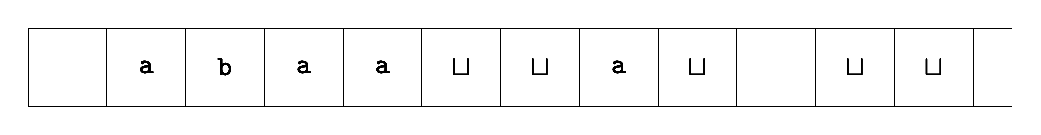
\begin{tikzpicture}

\draw (0.49999999999999994, 0.49999999999999994)
  node[draw, line width=0.01cm, , color=black,
       rounded corners=0cm, inner sep=0cm] {

\begin{minipage}[t][1.0cm]{1.0cm}
\mbox{}

\end{minipage}

};\draw (0.49999999999999994, 0.49999999999999994) node[color=black] {\texttt{\DOLLAR}};
\draw (1.5, 0.49999999999999994)
  node[draw, line width=0.01cm, , color=black,
       rounded corners=0cm, inner sep=0cm] {

\begin{minipage}[t][1.0cm]{1.0cm}
\mbox{}

\end{minipage}

};\draw (1.5, 0.49999999999999994) node[color=black] {\texttt{a}};
\draw (2.5, 0.49999999999999994)
  node[draw, line width=0.01cm, , color=black,
       rounded corners=0cm, inner sep=0cm] {

\begin{minipage}[t][1.0cm]{1.0cm}
\mbox{}

\end{minipage}

};\draw (2.5, 0.49999999999999994) node[color=black] {\texttt{b}};
\draw (3.5, 0.49999999999999994)
  node[draw, line width=0.01cm, , color=black,
       rounded corners=0cm, inner sep=0cm] {

\begin{minipage}[t][1.0cm]{1.0cm}
\mbox{}

\end{minipage}

};\draw (3.5, 0.49999999999999994) node[color=black] {\texttt{a}};
\draw (4.5, 0.49999999999999994)
  node[draw, line width=0.01cm, , color=black,
       rounded corners=0cm, inner sep=0cm] {

\begin{minipage}[t][1.0cm]{1.0cm}
\mbox{}

\end{minipage}

};\draw (4.5, 0.49999999999999994) node[color=black] {\texttt{a}};
\draw (5.5, 0.49999999999999994)
  node[draw, line width=0.01cm, , color=black,
       rounded corners=0cm, inner sep=0cm] {

\begin{minipage}[t][1.0cm]{1.0cm}
\mbox{}

\end{minipage}

};\draw (5.5, 0.49999999999999994) node[color=black] {\texttt{$\sqcup$}};
\draw (6.5, 0.49999999999999994)
  node[draw, line width=0.01cm, , color=black,
       rounded corners=0cm, inner sep=0cm] {

\begin{minipage}[t][1.0cm]{1.0cm}
\mbox{}

\end{minipage}

};\draw (6.5, 0.49999999999999994) node[color=black] {\texttt{$\sqcup$}};
\draw (7.5, 0.49999999999999994)
  node[draw, line width=0.01cm, , color=black,
       rounded corners=0cm, inner sep=0cm] {

\begin{minipage}[t][1.0cm]{1.0cm}
\mbox{}

\end{minipage}

};\draw (7.5, 0.49999999999999994) node[color=black] {\texttt{a}};
\draw (8.5, 0.49999999999999994)
  node[draw, line width=0.01cm, , color=black,
       rounded corners=0cm, inner sep=0cm] {

\begin{minipage}[t][1.0cm]{1.0cm}
\mbox{}

\end{minipage}

};\draw (8.5, 0.49999999999999994) node[color=black] {\texttt{$\sqcup$}};
\draw (9.5, 0.49999999999999994)
  node[draw, line width=0.01cm, , color=black,
       rounded corners=0cm, inner sep=0cm] {

\begin{minipage}[t][1.0cm]{1.0cm}
\mbox{}

\end{minipage}

};\draw (9.5, 0.49999999999999994) node[color=black] {\texttt{$\EOT$}};
\draw (10.5, 0.49999999999999994)
  node[draw, line width=0.01cm, , color=black,
       rounded corners=0cm, inner sep=0cm] {

\begin{minipage}[t][1.0cm]{1.0cm}
\mbox{}

\end{minipage}

};\draw (10.5, 0.49999999999999994) node[color=black] {\texttt{$\sqcup$}};
\draw (11.5, 0.49999999999999994)
  node[draw, line width=0.01cm, , color=black,
       rounded corners=0cm, inner sep=0cm] {

\begin{minipage}[t][1.0cm]{1.0cm}
\mbox{}

\end{minipage}

};\draw (11.5, 0.49999999999999994) node[color=black] {\texttt{$\sqcup$}};
\draw (0.49999999999999994, 0.49999999999999994)
  node[draw, line width=0.01cm, , color=black,
       rounded corners=0cm, inner sep=0cm] {

\begin{minipage}[t][1.0cm]{1.0cm}
\mbox{}

\end{minipage}

};\draw (0.49999999999999994, 0.49999999999999994) node[color=black] {\texttt{\DOLLAR}};
\draw (1.5, 0.49999999999999994)
  node[draw, line width=0.01cm, , color=black,
       rounded corners=0cm, inner sep=0cm] {

\begin{minipage}[t][1.0cm]{1.0cm}
\mbox{}

\end{minipage}

};\draw (1.5, 0.49999999999999994) node[color=black] {\texttt{a}};
\draw (2.5, 0.49999999999999994)
  node[draw, line width=0.01cm, , color=black,
       rounded corners=0cm, inner sep=0cm] {

\begin{minipage}[t][1.0cm]{1.0cm}
\mbox{}

\end{minipage}

};\draw (2.5, 0.49999999999999994) node[color=black] {\texttt{b}};
\draw (3.5, 0.49999999999999994)
  node[draw, line width=0.01cm, , color=black,
       rounded corners=0cm, inner sep=0cm] {

\begin{minipage}[t][1.0cm]{1.0cm}
\mbox{}

\end{minipage}

};\draw (3.5, 0.49999999999999994) node[color=black] {\texttt{a}};
\draw (4.5, 0.49999999999999994)
  node[draw, line width=0.01cm, , color=black,
       rounded corners=0cm, inner sep=0cm] {

\begin{minipage}[t][1.0cm]{1.0cm}
\mbox{}

\end{minipage}

};\draw (4.5, 0.49999999999999994) node[color=black] {\texttt{a}};
\draw (5.5, 0.49999999999999994)
  node[draw, line width=0.01cm, , color=black,
       rounded corners=0cm, inner sep=0cm] {

\begin{minipage}[t][1.0cm]{1.0cm}
\mbox{}

\end{minipage}

};\draw (5.5, 0.49999999999999994) node[color=black] {\texttt{$\sqcup$}};
\draw (6.5, 0.49999999999999994)
  node[draw, line width=0.01cm, , color=black,
       rounded corners=0cm, inner sep=0cm] {

\begin{minipage}[t][1.0cm]{1.0cm}
\mbox{}

\end{minipage}

};\draw (6.5, 0.49999999999999994) node[color=black] {\texttt{$\sqcup$}};
\draw (7.5, 0.49999999999999994)
  node[draw, line width=0.01cm, , color=black,
       rounded corners=0cm, inner sep=0cm] {

\begin{minipage}[t][1.0cm]{1.0cm}
\mbox{}

\end{minipage}

};\draw (7.5, 0.49999999999999994) node[color=black] {\texttt{a}};
\draw (8.5, 0.49999999999999994)
  node[draw, line width=0.01cm, , color=black,
       rounded corners=0cm, inner sep=0cm] {

\begin{minipage}[t][1.0cm]{1.0cm}
\mbox{}

\end{minipage}

};\draw (8.5, 0.49999999999999994) node[color=black] {\texttt{$\sqcup$}};
\draw (9.5, 0.49999999999999994)
  node[draw, line width=0.01cm, , color=black,
       rounded corners=0cm, inner sep=0cm] {

\begin{minipage}[t][1.0cm]{1.0cm}
\mbox{}

\end{minipage}

};\draw (9.5, 0.49999999999999994) node[color=black] {\texttt{$\EOT$}};
\draw (10.5, 0.49999999999999994)
  node[draw, line width=0.01cm, , color=black,
       rounded corners=0cm, inner sep=0cm] {

\begin{minipage}[t][1.0cm]{1.0cm}
\mbox{}

\end{minipage}

};\draw (10.5, 0.49999999999999994) node[color=black] {\texttt{$\sqcup$}};
\draw (11.5, 0.49999999999999994)
  node[draw, line width=0.01cm, , color=black,
       rounded corners=0cm, inner sep=0cm] {

\begin{minipage}[t][1.0cm]{1.0cm}
\mbox{}

\end{minipage}

};\draw (11.5, 0.49999999999999994) node[color=black] {\texttt{$\sqcup$}};
\draw (0.49999999999999994, 0.49999999999999994)
  node[draw, line width=0.01cm, , color=black,
       rounded corners=0cm, inner sep=0cm] {

\begin{minipage}[t][1.0cm]{1.0cm}
\mbox{}

\end{minipage}

};\draw (0.49999999999999994, 0.49999999999999994) node[color=black] {\texttt{\DOLLAR}};
\draw (1.5, 0.49999999999999994)
  node[draw, line width=0.01cm, , color=black,
       rounded corners=0cm, inner sep=0cm] {

\begin{minipage}[t][1.0cm]{1.0cm}
\mbox{}

\end{minipage}

};\draw (1.5, 0.49999999999999994) node[color=black] {\texttt{a}};
\draw (2.5, 0.49999999999999994)
  node[draw, line width=0.01cm, , color=black,
       rounded corners=0cm, inner sep=0cm] {

\begin{minipage}[t][1.0cm]{1.0cm}
\mbox{}

\end{minipage}

};\draw (2.5, 0.49999999999999994) node[color=black] {\texttt{b}};
\draw (3.5, 0.49999999999999994)
  node[draw, line width=0.01cm, , color=black,
       rounded corners=0cm, inner sep=0cm] {

\begin{minipage}[t][1.0cm]{1.0cm}
\mbox{}

\end{minipage}

};\draw (3.5, 0.49999999999999994) node[color=black] {\texttt{a}};
\draw (4.5, 0.49999999999999994)
  node[draw, line width=0.01cm, , color=black,
       rounded corners=0cm, inner sep=0cm] {

\begin{minipage}[t][1.0cm]{1.0cm}
\mbox{}

\end{minipage}

};\draw (4.5, 0.49999999999999994) node[color=black] {\texttt{a}};
\draw (5.5, 0.49999999999999994)
  node[draw, line width=0.01cm, , color=black,
       rounded corners=0cm, inner sep=0cm] {

\begin{minipage}[t][1.0cm]{1.0cm}
\mbox{}

\end{minipage}

};\draw (5.5, 0.49999999999999994) node[color=black] {\texttt{$\sqcup$}};
\draw (6.5, 0.49999999999999994)
  node[draw, line width=0.01cm, , color=black,
       rounded corners=0cm, inner sep=0cm] {

\begin{minipage}[t][1.0cm]{1.0cm}
\mbox{}

\end{minipage}

};\draw (6.5, 0.49999999999999994) node[color=black] {\texttt{$\sqcup$}};
\draw (7.5, 0.49999999999999994)
  node[draw, line width=0.01cm, , color=black,
       rounded corners=0cm, inner sep=0cm] {

\begin{minipage}[t][1.0cm]{1.0cm}
\mbox{}

\end{minipage}

};\draw (7.5, 0.49999999999999994) node[color=black] {\texttt{a}};
\draw (8.5, 0.49999999999999994)
  node[draw, line width=0.01cm, , color=black,
       rounded corners=0cm, inner sep=0cm] {

\begin{minipage}[t][1.0cm]{1.0cm}
\mbox{}

\end{minipage}

};\draw (8.5, 0.49999999999999994) node[color=black] {\texttt{$\sqcup$}};
\draw (9.5, 0.49999999999999994)
  node[draw, line width=0.01cm, , color=black,
       rounded corners=0cm, inner sep=0cm] {

\begin{minipage}[t][1.0cm]{1.0cm}
\mbox{}

\end{minipage}

};\draw (9.5, 0.49999999999999994) node[color=black] {\texttt{$\EOT$}};
\draw (10.5, 0.49999999999999994)
  node[draw, line width=0.01cm, , color=black,
       rounded corners=0cm, inner sep=0cm] {

\begin{minipage}[t][1.0cm]{1.0cm}
\mbox{}

\end{minipage}

};\draw (10.5, 0.49999999999999994) node[color=black] {\texttt{$\sqcup$}};
\draw (11.5, 0.49999999999999994)
  node[draw, line width=0.01cm, , color=black,
       rounded corners=0cm, inner sep=0cm] {

\begin{minipage}[t][1.0cm]{1.0cm}
\mbox{}

\end{minipage}

};\draw (11.5, 0.49999999999999994) node[color=black] {\texttt{$\sqcup$}};
\draw (0.49999999999999994, 0.49999999999999994)
  node[draw, line width=0.01cm, , color=black,
       rounded corners=0cm, inner sep=0cm] {

\begin{minipage}[t][1.0cm]{1.0cm}
\mbox{}

\end{minipage}

};\draw (0.49999999999999994, 0.49999999999999994) node[color=black] {\texttt{\DOLLAR}};
\draw (1.5, 0.49999999999999994)
  node[draw, line width=0.01cm, , color=black,
       rounded corners=0cm, inner sep=0cm] {

\begin{minipage}[t][1.0cm]{1.0cm}
\mbox{}

\end{minipage}

};\draw (1.5, 0.49999999999999994) node[color=black] {\texttt{a}};
\draw (2.5, 0.49999999999999994)
  node[draw, line width=0.01cm, , color=black,
       rounded corners=0cm, inner sep=0cm] {

\begin{minipage}[t][1.0cm]{1.0cm}
\mbox{}

\end{minipage}

};\draw (2.5, 0.49999999999999994) node[color=black] {\texttt{b}};
\draw (3.5, 0.49999999999999994)
  node[draw, line width=0.01cm, , color=black,
       rounded corners=0cm, inner sep=0cm] {

\begin{minipage}[t][1.0cm]{1.0cm}
\mbox{}

\end{minipage}

};\draw (3.5, 0.49999999999999994) node[color=black] {\texttt{a}};
\draw (4.5, 0.49999999999999994)
  node[draw, line width=0.01cm, , color=black,
       rounded corners=0cm, inner sep=0cm] {

\begin{minipage}[t][1.0cm]{1.0cm}
\mbox{}

\end{minipage}

};\draw (4.5, 0.49999999999999994) node[color=black] {\texttt{a}};
\draw (5.5, 0.49999999999999994)
  node[draw, line width=0.01cm, , color=black,
       rounded corners=0cm, inner sep=0cm] {

\begin{minipage}[t][1.0cm]{1.0cm}
\mbox{}

\end{minipage}

};\draw (5.5, 0.49999999999999994) node[color=black] {\texttt{$\sqcup$}};
\draw (6.5, 0.49999999999999994)
  node[draw, line width=0.01cm, , color=black,
       rounded corners=0cm, inner sep=0cm] {

\begin{minipage}[t][1.0cm]{1.0cm}
\mbox{}

\end{minipage}

};\draw (6.5, 0.49999999999999994) node[color=black] {\texttt{$\sqcup$}};
\draw (7.5, 0.49999999999999994)
  node[draw, line width=0.01cm, , color=black,
       rounded corners=0cm, inner sep=0cm] {

\begin{minipage}[t][1.0cm]{1.0cm}
\mbox{}

\end{minipage}

};\draw (7.5, 0.49999999999999994) node[color=black] {\texttt{a}};
\draw (8.5, 0.49999999999999994)
  node[draw, line width=0.01cm, , color=black,
       rounded corners=0cm, inner sep=0cm] {

\begin{minipage}[t][1.0cm]{1.0cm}
\mbox{}

\end{minipage}

};\draw (8.5, 0.49999999999999994) node[color=black] {\texttt{$\sqcup$}};
\draw (9.5, 0.49999999999999994)
  node[draw, line width=0.01cm, , color=black,
       rounded corners=0cm, inner sep=0cm] {

\begin{minipage}[t][1.0cm]{1.0cm}
\mbox{}

\end{minipage}

};\draw (9.5, 0.49999999999999994) node[color=black] {\texttt{$\EOT$}};
\draw (10.5, 0.49999999999999994)
  node[draw, line width=0.01cm, , color=black,
       rounded corners=0cm, inner sep=0cm] {

\begin{minipage}[t][1.0cm]{1.0cm}
\mbox{}

\end{minipage}

};\draw (10.5, 0.49999999999999994) node[color=black] {\texttt{$\sqcup$}};
\draw (11.5, 0.49999999999999994)
  node[draw, line width=0.01cm, , color=black,
       rounded corners=0cm, inner sep=0cm] {

\begin{minipage}[t][1.0cm]{1.0cm}
\mbox{}

\end{minipage}

};\draw (11.5, 0.49999999999999994) node[color=black] {\texttt{$\sqcup$}};
\draw (0.49999999999999994, 0.49999999999999994)
  node[draw, line width=0.01cm, , color=black,
       rounded corners=0cm, inner sep=0cm] {

\begin{minipage}[t][1.0cm]{1.0cm}
\mbox{}

\end{minipage}

};\draw (0.49999999999999994, 0.49999999999999994) node[color=black] {\texttt{\DOLLAR}};
\draw (1.5, 0.49999999999999994)
  node[draw, line width=0.01cm, , color=black,
       rounded corners=0cm, inner sep=0cm] {

\begin{minipage}[t][1.0cm]{1.0cm}
\mbox{}

\end{minipage}

};\draw (1.5, 0.49999999999999994) node[color=black] {\texttt{a}};
\draw (2.5, 0.49999999999999994)
  node[draw, line width=0.01cm, , color=black,
       rounded corners=0cm, inner sep=0cm] {

\begin{minipage}[t][1.0cm]{1.0cm}
\mbox{}

\end{minipage}

};\draw (2.5, 0.49999999999999994) node[color=black] {\texttt{b}};
\draw (3.5, 0.49999999999999994)
  node[draw, line width=0.01cm, , color=black,
       rounded corners=0cm, inner sep=0cm] {

\begin{minipage}[t][1.0cm]{1.0cm}
\mbox{}

\end{minipage}

};\draw (3.5, 0.49999999999999994) node[color=black] {\texttt{a}};
\draw (4.5, 0.49999999999999994)
  node[draw, line width=0.01cm, , color=black,
       rounded corners=0cm, inner sep=0cm] {

\begin{minipage}[t][1.0cm]{1.0cm}
\mbox{}

\end{minipage}

};\draw (4.5, 0.49999999999999994) node[color=black] {\texttt{a}};
\draw (5.5, 0.49999999999999994)
  node[draw, line width=0.01cm, , color=black,
       rounded corners=0cm, inner sep=0cm] {

\begin{minipage}[t][1.0cm]{1.0cm}
\mbox{}

\end{minipage}

};\draw (5.5, 0.49999999999999994) node[color=black] {\texttt{$\sqcup$}};
\draw (6.5, 0.49999999999999994)
  node[draw, line width=0.01cm, , color=black,
       rounded corners=0cm, inner sep=0cm] {

\begin{minipage}[t][1.0cm]{1.0cm}
\mbox{}

\end{minipage}

};\draw (6.5, 0.49999999999999994) node[color=black] {\texttt{$\sqcup$}};
\draw (7.5, 0.49999999999999994)
  node[draw, line width=0.01cm, , color=black,
       rounded corners=0cm, inner sep=0cm] {

\begin{minipage}[t][1.0cm]{1.0cm}
\mbox{}

\end{minipage}

};\draw (7.5, 0.49999999999999994) node[color=black] {\texttt{a}};
\draw (8.5, 0.49999999999999994)
  node[draw, line width=0.01cm, , color=black,
       rounded corners=0cm, inner sep=0cm] {

\begin{minipage}[t][1.0cm]{1.0cm}
\mbox{}

\end{minipage}

};\draw (8.5, 0.49999999999999994) node[color=black] {\texttt{$\sqcup$}};
\draw (9.5, 0.49999999999999994)
  node[draw, line width=0.01cm, , color=black,
       rounded corners=0cm, inner sep=0cm] {

\begin{minipage}[t][1.0cm]{1.0cm}
\mbox{}

\end{minipage}

};\draw (9.5, 0.49999999999999994) node[color=black] {\texttt{$\EOT$}};
\draw (10.5, 0.49999999999999994)
  node[draw, line width=0.01cm, , color=black,
       rounded corners=0cm, inner sep=0cm] {

\begin{minipage}[t][1.0cm]{1.0cm}
\mbox{}

\end{minipage}

};\draw (10.5, 0.49999999999999994) node[color=black] {\texttt{$\sqcup$}};
\draw (11.5, 0.49999999999999994)
  node[draw, line width=0.01cm, , color=black,
       rounded corners=0cm, inner sep=0cm] {

\begin{minipage}[t][1.0cm]{1.0cm}
\mbox{}

\end{minipage}

};\draw (11.5, 0.49999999999999994) node[color=black] {\texttt{$\sqcup$}};
\draw (0.49999999999999994, 0.49999999999999994)
  node[draw, line width=0.01cm, , color=black,
       rounded corners=0cm, inner sep=0cm] {

\begin{minipage}[t][1.0cm]{1.0cm}
\mbox{}

\end{minipage}

};\draw (0.49999999999999994, 0.49999999999999994) node[color=black] {\texttt{\DOLLAR}};
\draw (1.5, 0.49999999999999994)
  node[draw, line width=0.01cm, , color=black,
       rounded corners=0cm, inner sep=0cm] {

\begin{minipage}[t][1.0cm]{1.0cm}
\mbox{}

\end{minipage}

};\draw (1.5, 0.49999999999999994) node[color=black] {\texttt{a}};
\draw (2.5, 0.49999999999999994)
  node[draw, line width=0.01cm, , color=black,
       rounded corners=0cm, inner sep=0cm] {

\begin{minipage}[t][1.0cm]{1.0cm}
\mbox{}

\end{minipage}

};\draw (2.5, 0.49999999999999994) node[color=black] {\texttt{b}};
\draw (3.5, 0.49999999999999994)
  node[draw, line width=0.01cm, , color=black,
       rounded corners=0cm, inner sep=0cm] {

\begin{minipage}[t][1.0cm]{1.0cm}
\mbox{}

\end{minipage}

};\draw (3.5, 0.49999999999999994) node[color=black] {\texttt{a}};
\draw (4.5, 0.49999999999999994)
  node[draw, line width=0.01cm, , color=black,
       rounded corners=0cm, inner sep=0cm] {

\begin{minipage}[t][1.0cm]{1.0cm}
\mbox{}

\end{minipage}

};\draw (4.5, 0.49999999999999994) node[color=black] {\texttt{a}};
\draw (5.5, 0.49999999999999994)
  node[draw, line width=0.01cm, , color=black,
       rounded corners=0cm, inner sep=0cm] {

\begin{minipage}[t][1.0cm]{1.0cm}
\mbox{}

\end{minipage}

};\draw (5.5, 0.49999999999999994) node[color=black] {\texttt{$\sqcup$}};
\draw (6.5, 0.49999999999999994)
  node[draw, line width=0.01cm, , color=black,
       rounded corners=0cm, inner sep=0cm] {

\begin{minipage}[t][1.0cm]{1.0cm}
\mbox{}

\end{minipage}

};\draw (6.5, 0.49999999999999994) node[color=black] {\texttt{$\sqcup$}};
\draw (7.5, 0.49999999999999994)
  node[draw, line width=0.01cm, , color=black,
       rounded corners=0cm, inner sep=0cm] {

\begin{minipage}[t][1.0cm]{1.0cm}
\mbox{}

\end{minipage}

};\draw (7.5, 0.49999999999999994) node[color=black] {\texttt{a}};
\draw (8.5, 0.49999999999999994)
  node[draw, line width=0.01cm, , color=black,
       rounded corners=0cm, inner sep=0cm] {

\begin{minipage}[t][1.0cm]{1.0cm}
\mbox{}

\end{minipage}

};\draw (8.5, 0.49999999999999994) node[color=black] {\texttt{$\sqcup$}};
\draw (9.5, 0.49999999999999994)
  node[draw, line width=0.01cm, , color=black,
       rounded corners=0cm, inner sep=0cm] {

\begin{minipage}[t][1.0cm]{1.0cm}
\mbox{}

\end{minipage}

};\draw (9.5, 0.49999999999999994) node[color=black] {\texttt{$\EOT$}};
\draw (10.5, 0.49999999999999994)
  node[draw, line width=0.01cm, , color=black,
       rounded corners=0cm, inner sep=0cm] {

\begin{minipage}[t][1.0cm]{1.0cm}
\mbox{}

\end{minipage}

};\draw (10.5, 0.49999999999999994) node[color=black] {\texttt{$\sqcup$}};
\draw (11.5, 0.49999999999999994)
  node[draw, line width=0.01cm, , color=black,
       rounded corners=0cm, inner sep=0cm] {

\begin{minipage}[t][1.0cm]{1.0cm}
\mbox{}

\end{minipage}

};\draw (11.5, 0.49999999999999994) node[color=black] {\texttt{$\sqcup$}};
\draw (0.49999999999999994, 0.49999999999999994)
  node[draw, line width=0.01cm, , color=black,
       rounded corners=0cm, inner sep=0cm] {

\begin{minipage}[t][1.0cm]{1.0cm}
\mbox{}

\end{minipage}

};\draw (0.49999999999999994, 0.49999999999999994) node[color=black] {\texttt{\DOLLAR}};
\draw (1.5, 0.49999999999999994)
  node[draw, line width=0.01cm, , color=black,
       rounded corners=0cm, inner sep=0cm] {

\begin{minipage}[t][1.0cm]{1.0cm}
\mbox{}

\end{minipage}

};\draw (1.5, 0.49999999999999994) node[color=black] {\texttt{a}};
\draw (2.5, 0.49999999999999994)
  node[draw, line width=0.01cm, , color=black,
       rounded corners=0cm, inner sep=0cm] {

\begin{minipage}[t][1.0cm]{1.0cm}
\mbox{}

\end{minipage}

};\draw (2.5, 0.49999999999999994) node[color=black] {\texttt{b}};
\draw (3.5, 0.49999999999999994)
  node[draw, line width=0.01cm, , color=black,
       rounded corners=0cm, inner sep=0cm] {

\begin{minipage}[t][1.0cm]{1.0cm}
\mbox{}

\end{minipage}

};\draw (3.5, 0.49999999999999994) node[color=black] {\texttt{a}};
\draw (4.5, 0.49999999999999994)
  node[draw, line width=0.01cm, , color=black,
       rounded corners=0cm, inner sep=0cm] {

\begin{minipage}[t][1.0cm]{1.0cm}
\mbox{}

\end{minipage}

};\draw (4.5, 0.49999999999999994) node[color=black] {\texttt{a}};
\draw (5.5, 0.49999999999999994)
  node[draw, line width=0.01cm, , color=black,
       rounded corners=0cm, inner sep=0cm] {

\begin{minipage}[t][1.0cm]{1.0cm}
\mbox{}

\end{minipage}

};\draw (5.5, 0.49999999999999994) node[color=black] {\texttt{$\sqcup$}};
\draw (6.5, 0.49999999999999994)
  node[draw, line width=0.01cm, , color=black,
       rounded corners=0cm, inner sep=0cm] {

\begin{minipage}[t][1.0cm]{1.0cm}
\mbox{}

\end{minipage}

};\draw (6.5, 0.49999999999999994) node[color=black] {\texttt{$\sqcup$}};
\draw (7.5, 0.49999999999999994)
  node[draw, line width=0.01cm, , color=black,
       rounded corners=0cm, inner sep=0cm] {

\begin{minipage}[t][1.0cm]{1.0cm}
\mbox{}

\end{minipage}

};\draw (7.5, 0.49999999999999994) node[color=black] {\texttt{a}};
\draw (8.5, 0.49999999999999994)
  node[draw, line width=0.01cm, , color=black,
       rounded corners=0cm, inner sep=0cm] {

\begin{minipage}[t][1.0cm]{1.0cm}
\mbox{}

\end{minipage}

};\draw (8.5, 0.49999999999999994) node[color=black] {\texttt{$\sqcup$}};
\draw (9.5, 0.49999999999999994)
  node[draw, line width=0.01cm, , color=black,
       rounded corners=0cm, inner sep=0cm] {

\begin{minipage}[t][1.0cm]{1.0cm}
\mbox{}

\end{minipage}

};\draw (9.5, 0.49999999999999994) node[color=black] {\texttt{$\EOT$}};
\draw (10.5, 0.49999999999999994)
  node[draw, line width=0.01cm, , color=black,
       rounded corners=0cm, inner sep=0cm] {

\begin{minipage}[t][1.0cm]{1.0cm}
\mbox{}

\end{minipage}

};\draw (10.5, 0.49999999999999994) node[color=black] {\texttt{$\sqcup$}};
\draw (11.5, 0.49999999999999994)
  node[draw, line width=0.01cm, , color=black,
       rounded corners=0cm, inner sep=0cm] {

\begin{minipage}[t][1.0cm]{1.0cm}
\mbox{}

\end{minipage}

};\draw (11.5, 0.49999999999999994) node[color=black] {\texttt{$\sqcup$}};
\draw (0.49999999999999994, 0.49999999999999994)
  node[draw, line width=0.01cm, , color=black,
       rounded corners=0cm, inner sep=0cm] {

\begin{minipage}[t][1.0cm]{1.0cm}
\mbox{}

\end{minipage}

};\draw (0.49999999999999994, 0.49999999999999994) node[color=black] {\texttt{\DOLLAR}};
\draw (1.5, 0.49999999999999994)
  node[draw, line width=0.01cm, , color=black,
       rounded corners=0cm, inner sep=0cm] {

\begin{minipage}[t][1.0cm]{1.0cm}
\mbox{}

\end{minipage}

};\draw (1.5, 0.49999999999999994) node[color=black] {\texttt{a}};
\draw (2.5, 0.49999999999999994)
  node[draw, line width=0.01cm, , color=black,
       rounded corners=0cm, inner sep=0cm] {

\begin{minipage}[t][1.0cm]{1.0cm}
\mbox{}

\end{minipage}

};\draw (2.5, 0.49999999999999994) node[color=black] {\texttt{b}};
\draw (3.5, 0.49999999999999994)
  node[draw, line width=0.01cm, , color=black,
       rounded corners=0cm, inner sep=0cm] {

\begin{minipage}[t][1.0cm]{1.0cm}
\mbox{}

\end{minipage}

};\draw (3.5, 0.49999999999999994) node[color=black] {\texttt{a}};
\draw (4.5, 0.49999999999999994)
  node[draw, line width=0.01cm, , color=black,
       rounded corners=0cm, inner sep=0cm] {

\begin{minipage}[t][1.0cm]{1.0cm}
\mbox{}

\end{minipage}

};\draw (4.5, 0.49999999999999994) node[color=black] {\texttt{a}};
\draw (5.5, 0.49999999999999994)
  node[draw, line width=0.01cm, , color=black,
       rounded corners=0cm, inner sep=0cm] {

\begin{minipage}[t][1.0cm]{1.0cm}
\mbox{}

\end{minipage}

};\draw (5.5, 0.49999999999999994) node[color=black] {\texttt{$\sqcup$}};
\draw (6.5, 0.49999999999999994)
  node[draw, line width=0.01cm, , color=black,
       rounded corners=0cm, inner sep=0cm] {

\begin{minipage}[t][1.0cm]{1.0cm}
\mbox{}

\end{minipage}

};\draw (6.5, 0.49999999999999994) node[color=black] {\texttt{$\sqcup$}};
\draw (7.5, 0.49999999999999994)
  node[draw, line width=0.01cm, , color=black,
       rounded corners=0cm, inner sep=0cm] {

\begin{minipage}[t][1.0cm]{1.0cm}
\mbox{}

\end{minipage}

};\draw (7.5, 0.49999999999999994) node[color=black] {\texttt{a}};
\draw (8.5, 0.49999999999999994)
  node[draw, line width=0.01cm, , color=black,
       rounded corners=0cm, inner sep=0cm] {

\begin{minipage}[t][1.0cm]{1.0cm}
\mbox{}

\end{minipage}

};\draw (8.5, 0.49999999999999994) node[color=black] {\texttt{$\sqcup$}};
\draw (9.5, 0.49999999999999994)
  node[draw, line width=0.01cm, , color=black,
       rounded corners=0cm, inner sep=0cm] {

\begin{minipage}[t][1.0cm]{1.0cm}
\mbox{}

\end{minipage}

};\draw (9.5, 0.49999999999999994) node[color=black] {\texttt{$\EOT$}};
\draw (10.5, 0.49999999999999994)
  node[draw, line width=0.01cm, , color=black,
       rounded corners=0cm, inner sep=0cm] {

\begin{minipage}[t][1.0cm]{1.0cm}
\mbox{}

\end{minipage}

};\draw (10.5, 0.49999999999999994) node[color=black] {\texttt{$\sqcup$}};
\draw (11.5, 0.49999999999999994)
  node[draw, line width=0.01cm, , color=black,
       rounded corners=0cm, inner sep=0cm] {

\begin{minipage}[t][1.0cm]{1.0cm}
\mbox{}

\end{minipage}

};\draw (11.5, 0.49999999999999994) node[color=black] {\texttt{$\sqcup$}};
\draw (0.49999999999999994, 0.49999999999999994)
  node[draw, line width=0.01cm, , color=black,
       rounded corners=0cm, inner sep=0cm] {

\begin{minipage}[t][1.0cm]{1.0cm}
\mbox{}

\end{minipage}

};\draw (0.49999999999999994, 0.49999999999999994) node[color=black] {\texttt{\DOLLAR}};
\draw (1.5, 0.49999999999999994)
  node[draw, line width=0.01cm, , color=black,
       rounded corners=0cm, inner sep=0cm] {

\begin{minipage}[t][1.0cm]{1.0cm}
\mbox{}

\end{minipage}

};\draw (1.5, 0.49999999999999994) node[color=black] {\texttt{a}};
\draw (2.5, 0.49999999999999994)
  node[draw, line width=0.01cm, , color=black,
       rounded corners=0cm, inner sep=0cm] {

\begin{minipage}[t][1.0cm]{1.0cm}
\mbox{}

\end{minipage}

};\draw (2.5, 0.49999999999999994) node[color=black] {\texttt{b}};
\draw (3.5, 0.49999999999999994)
  node[draw, line width=0.01cm, , color=black,
       rounded corners=0cm, inner sep=0cm] {

\begin{minipage}[t][1.0cm]{1.0cm}
\mbox{}

\end{minipage}

};\draw (3.5, 0.49999999999999994) node[color=black] {\texttt{a}};
\draw (4.5, 0.49999999999999994)
  node[draw, line width=0.01cm, , color=black,
       rounded corners=0cm, inner sep=0cm] {

\begin{minipage}[t][1.0cm]{1.0cm}
\mbox{}

\end{minipage}

};\draw (4.5, 0.49999999999999994) node[color=black] {\texttt{a}};
\draw (5.5, 0.49999999999999994)
  node[draw, line width=0.01cm, , color=black,
       rounded corners=0cm, inner sep=0cm] {

\begin{minipage}[t][1.0cm]{1.0cm}
\mbox{}

\end{minipage}

};\draw (5.5, 0.49999999999999994) node[color=black] {\texttt{$\sqcup$}};
\draw (6.5, 0.49999999999999994)
  node[draw, line width=0.01cm, , color=black,
       rounded corners=0cm, inner sep=0cm] {

\begin{minipage}[t][1.0cm]{1.0cm}
\mbox{}

\end{minipage}

};\draw (6.5, 0.49999999999999994) node[color=black] {\texttt{$\sqcup$}};
\draw (7.5, 0.49999999999999994)
  node[draw, line width=0.01cm, , color=black,
       rounded corners=0cm, inner sep=0cm] {

\begin{minipage}[t][1.0cm]{1.0cm}
\mbox{}

\end{minipage}

};\draw (7.5, 0.49999999999999994) node[color=black] {\texttt{a}};
\draw (8.5, 0.49999999999999994)
  node[draw, line width=0.01cm, , color=black,
       rounded corners=0cm, inner sep=0cm] {

\begin{minipage}[t][1.0cm]{1.0cm}
\mbox{}

\end{minipage}

};\draw (8.5, 0.49999999999999994) node[color=black] {\texttt{$\sqcup$}};
\draw (9.5, 0.49999999999999994)
  node[draw, line width=0.01cm, , color=black,
       rounded corners=0cm, inner sep=0cm] {

\begin{minipage}[t][1.0cm]{1.0cm}
\mbox{}

\end{minipage}

};\draw (9.5, 0.49999999999999994) node[color=black] {\texttt{$\EOT$}};
\draw (10.5, 0.49999999999999994)
  node[draw, line width=0.01cm, , color=black,
       rounded corners=0cm, inner sep=0cm] {

\begin{minipage}[t][1.0cm]{1.0cm}
\mbox{}

\end{minipage}

};\draw (10.5, 0.49999999999999994) node[color=black] {\texttt{$\sqcup$}};
\draw (11.5, 0.49999999999999994)
  node[draw, line width=0.01cm, , color=black,
       rounded corners=0cm, inner sep=0cm] {

\begin{minipage}[t][1.0cm]{1.0cm}
\mbox{}

\end{minipage}

};\draw (11.5, 0.49999999999999994) node[color=black] {\texttt{$\sqcup$}};
\draw (0.49999999999999994, 0.49999999999999994)
  node[draw, line width=0.01cm, , color=black,
       rounded corners=0cm, inner sep=0cm] {

\begin{minipage}[t][1.0cm]{1.0cm}
\mbox{}

\end{minipage}

};\draw (0.49999999999999994, 0.49999999999999994) node[color=black] {\texttt{\DOLLAR}};
\draw (1.5, 0.49999999999999994)
  node[draw, line width=0.01cm, , color=black,
       rounded corners=0cm, inner sep=0cm] {

\begin{minipage}[t][1.0cm]{1.0cm}
\mbox{}

\end{minipage}

};\draw (1.5, 0.49999999999999994) node[color=black] {\texttt{a}};
\draw (2.5, 0.49999999999999994)
  node[draw, line width=0.01cm, , color=black,
       rounded corners=0cm, inner sep=0cm] {

\begin{minipage}[t][1.0cm]{1.0cm}
\mbox{}

\end{minipage}

};\draw (2.5, 0.49999999999999994) node[color=black] {\texttt{b}};
\draw (3.5, 0.49999999999999994)
  node[draw, line width=0.01cm, , color=black,
       rounded corners=0cm, inner sep=0cm] {

\begin{minipage}[t][1.0cm]{1.0cm}
\mbox{}

\end{minipage}

};\draw (3.5, 0.49999999999999994) node[color=black] {\texttt{a}};
\draw (4.5, 0.49999999999999994)
  node[draw, line width=0.01cm, , color=black,
       rounded corners=0cm, inner sep=0cm] {

\begin{minipage}[t][1.0cm]{1.0cm}
\mbox{}

\end{minipage}

};\draw (4.5, 0.49999999999999994) node[color=black] {\texttt{a}};
\draw (5.5, 0.49999999999999994)
  node[draw, line width=0.01cm, , color=black,
       rounded corners=0cm, inner sep=0cm] {

\begin{minipage}[t][1.0cm]{1.0cm}
\mbox{}

\end{minipage}

};\draw (5.5, 0.49999999999999994) node[color=black] {\texttt{$\sqcup$}};
\draw (6.5, 0.49999999999999994)
  node[draw, line width=0.01cm, , color=black,
       rounded corners=0cm, inner sep=0cm] {

\begin{minipage}[t][1.0cm]{1.0cm}
\mbox{}

\end{minipage}

};\draw (6.5, 0.49999999999999994) node[color=black] {\texttt{$\sqcup$}};
\draw (7.5, 0.49999999999999994)
  node[draw, line width=0.01cm, , color=black,
       rounded corners=0cm, inner sep=0cm] {

\begin{minipage}[t][1.0cm]{1.0cm}
\mbox{}

\end{minipage}

};\draw (7.5, 0.49999999999999994) node[color=black] {\texttt{a}};
\draw (8.5, 0.49999999999999994)
  node[draw, line width=0.01cm, , color=black,
       rounded corners=0cm, inner sep=0cm] {

\begin{minipage}[t][1.0cm]{1.0cm}
\mbox{}

\end{minipage}

};\draw (8.5, 0.49999999999999994) node[color=black] {\texttt{$\sqcup$}};
\draw (9.5, 0.49999999999999994)
  node[draw, line width=0.01cm, , color=black,
       rounded corners=0cm, inner sep=0cm] {

\begin{minipage}[t][1.0cm]{1.0cm}
\mbox{}

\end{minipage}

};\draw (9.5, 0.49999999999999994) node[color=black] {\texttt{$\EOT$}};
\draw (10.5, 0.49999999999999994)
  node[draw, line width=0.01cm, , color=black,
       rounded corners=0cm, inner sep=0cm] {

\begin{minipage}[t][1.0cm]{1.0cm}
\mbox{}

\end{minipage}

};\draw (10.5, 0.49999999999999994) node[color=black] {\texttt{$\sqcup$}};
\draw (11.5, 0.49999999999999994)
  node[draw, line width=0.01cm, , color=black,
       rounded corners=0cm, inner sep=0cm] {

\begin{minipage}[t][1.0cm]{1.0cm}
\mbox{}

\end{minipage}

};\draw (11.5, 0.49999999999999994) node[color=black] {\texttt{$\sqcup$}};
\draw (0.49999999999999994, 0.49999999999999994)
  node[draw, line width=0.01cm, , color=black,
       rounded corners=0cm, inner sep=0cm] {

\begin{minipage}[t][1.0cm]{1.0cm}
\mbox{}

\end{minipage}

};\draw (0.49999999999999994, 0.49999999999999994) node[color=black] {\texttt{\DOLLAR}};
\draw (1.5, 0.49999999999999994)
  node[draw, line width=0.01cm, , color=black,
       rounded corners=0cm, inner sep=0cm] {

\begin{minipage}[t][1.0cm]{1.0cm}
\mbox{}

\end{minipage}

};\draw (1.5, 0.49999999999999994) node[color=black] {\texttt{a}};
\draw (2.5, 0.49999999999999994)
  node[draw, line width=0.01cm, , color=black,
       rounded corners=0cm, inner sep=0cm] {

\begin{minipage}[t][1.0cm]{1.0cm}
\mbox{}

\end{minipage}

};\draw (2.5, 0.49999999999999994) node[color=black] {\texttt{b}};
\draw (3.5, 0.49999999999999994)
  node[draw, line width=0.01cm, , color=black,
       rounded corners=0cm, inner sep=0cm] {

\begin{minipage}[t][1.0cm]{1.0cm}
\mbox{}

\end{minipage}

};\draw (3.5, 0.49999999999999994) node[color=black] {\texttt{a}};
\draw (4.5, 0.49999999999999994)
  node[draw, line width=0.01cm, , color=black,
       rounded corners=0cm, inner sep=0cm] {

\begin{minipage}[t][1.0cm]{1.0cm}
\mbox{}

\end{minipage}

};\draw (4.5, 0.49999999999999994) node[color=black] {\texttt{a}};
\draw (5.5, 0.49999999999999994)
  node[draw, line width=0.01cm, , color=black,
       rounded corners=0cm, inner sep=0cm] {

\begin{minipage}[t][1.0cm]{1.0cm}
\mbox{}

\end{minipage}

};\draw (5.5, 0.49999999999999994) node[color=black] {\texttt{$\sqcup$}};
\draw (6.5, 0.49999999999999994)
  node[draw, line width=0.01cm, , color=black,
       rounded corners=0cm, inner sep=0cm] {

\begin{minipage}[t][1.0cm]{1.0cm}
\mbox{}

\end{minipage}

};\draw (6.5, 0.49999999999999994) node[color=black] {\texttt{$\sqcup$}};
\draw (7.5, 0.49999999999999994)
  node[draw, line width=0.01cm, , color=black,
       rounded corners=0cm, inner sep=0cm] {

\begin{minipage}[t][1.0cm]{1.0cm}
\mbox{}

\end{minipage}

};\draw (7.5, 0.49999999999999994) node[color=black] {\texttt{a}};
\draw (8.5, 0.49999999999999994)
  node[draw, line width=0.01cm, , color=black,
       rounded corners=0cm, inner sep=0cm] {

\begin{minipage}[t][1.0cm]{1.0cm}
\mbox{}

\end{minipage}

};\draw (8.5, 0.49999999999999994) node[color=black] {\texttt{$\sqcup$}};
\draw (9.5, 0.49999999999999994)
  node[draw, line width=0.01cm, , color=black,
       rounded corners=0cm, inner sep=0cm] {

\begin{minipage}[t][1.0cm]{1.0cm}
\mbox{}

\end{minipage}

};\draw (9.5, 0.49999999999999994) node[color=black] {\texttt{$\EOT$}};
\draw (10.5, 0.49999999999999994)
  node[draw, line width=0.01cm, , color=black,
       rounded corners=0cm, inner sep=0cm] {

\begin{minipage}[t][1.0cm]{1.0cm}
\mbox{}

\end{minipage}

};\draw (10.5, 0.49999999999999994) node[color=black] {\texttt{$\sqcup$}};
\draw (11.5, 0.49999999999999994)
  node[draw, line width=0.01cm, , color=black,
       rounded corners=0cm, inner sep=0cm] {

\begin{minipage}[t][1.0cm]{1.0cm}
\mbox{}

\end{minipage}

};\draw (11.5, 0.49999999999999994) node[color=black] {\texttt{$\sqcup$}};
\draw (0.49999999999999994, 0.49999999999999994)
  node[draw, line width=0.01cm, , color=black,
       rounded corners=0cm, inner sep=0cm] {

\begin{minipage}[t][1.0cm]{1.0cm}
\mbox{}

\end{minipage}

};\draw (0.49999999999999994, 0.49999999999999994) node[color=black] {\texttt{\DOLLAR}};
\draw (1.5, 0.49999999999999994)
  node[draw, line width=0.01cm, , color=black,
       rounded corners=0cm, inner sep=0cm] {

\begin{minipage}[t][1.0cm]{1.0cm}
\mbox{}

\end{minipage}

};\draw (1.5, 0.49999999999999994) node[color=black] {\texttt{a}};
\draw (2.5, 0.49999999999999994)
  node[draw, line width=0.01cm, , color=black,
       rounded corners=0cm, inner sep=0cm] {

\begin{minipage}[t][1.0cm]{1.0cm}
\mbox{}

\end{minipage}

};\draw (2.5, 0.49999999999999994) node[color=black] {\texttt{b}};
\draw (3.5, 0.49999999999999994)
  node[draw, line width=0.01cm, , color=black,
       rounded corners=0cm, inner sep=0cm] {

\begin{minipage}[t][1.0cm]{1.0cm}
\mbox{}

\end{minipage}

};\draw (3.5, 0.49999999999999994) node[color=black] {\texttt{a}};
\draw (4.5, 0.49999999999999994)
  node[draw, line width=0.01cm, , color=black,
       rounded corners=0cm, inner sep=0cm] {

\begin{minipage}[t][1.0cm]{1.0cm}
\mbox{}

\end{minipage}

};\draw (4.5, 0.49999999999999994) node[color=black] {\texttt{a}};
\draw (5.5, 0.49999999999999994)
  node[draw, line width=0.01cm, , color=black,
       rounded corners=0cm, inner sep=0cm] {

\begin{minipage}[t][1.0cm]{1.0cm}
\mbox{}

\end{minipage}

};\draw (5.5, 0.49999999999999994) node[color=black] {\texttt{$\sqcup$}};
\draw (6.5, 0.49999999999999994)
  node[draw, line width=0.01cm, , color=black,
       rounded corners=0cm, inner sep=0cm] {

\begin{minipage}[t][1.0cm]{1.0cm}
\mbox{}

\end{minipage}

};\draw (6.5, 0.49999999999999994) node[color=black] {\texttt{$\sqcup$}};
\draw (7.5, 0.49999999999999994)
  node[draw, line width=0.01cm, , color=black,
       rounded corners=0cm, inner sep=0cm] {

\begin{minipage}[t][1.0cm]{1.0cm}
\mbox{}

\end{minipage}

};\draw (7.5, 0.49999999999999994) node[color=black] {\texttt{a}};
\draw (8.5, 0.49999999999999994)
  node[draw, line width=0.01cm, , color=black,
       rounded corners=0cm, inner sep=0cm] {

\begin{minipage}[t][1.0cm]{1.0cm}
\mbox{}

\end{minipage}

};\draw (8.5, 0.49999999999999994) node[color=black] {\texttt{$\sqcup$}};
\draw (9.5, 0.49999999999999994)
  node[draw, line width=0.01cm, , color=black,
       rounded corners=0cm, inner sep=0cm] {

\begin{minipage}[t][1.0cm]{1.0cm}
\mbox{}

\end{minipage}

};\draw (9.5, 0.49999999999999994) node[color=black] {\texttt{$\EOT$}};
\draw (10.5, 0.49999999999999994)
  node[draw, line width=0.01cm, , color=black,
       rounded corners=0cm, inner sep=0cm] {

\begin{minipage}[t][1.0cm]{1.0cm}
\mbox{}

\end{minipage}

};\draw (10.5, 0.49999999999999994) node[color=black] {\texttt{$\sqcup$}};
\draw (11.5, 0.49999999999999994)
  node[draw, line width=0.01cm, , color=black,
       rounded corners=0cm, inner sep=0cm] {

\begin{minipage}[t][1.0cm]{1.0cm}
\mbox{}

\end{minipage}

};\draw (11.5, 0.49999999999999994) node[color=black] {\texttt{$\sqcup$}};\draw[line width=0.01cm,black] (12.0,1.0) to  (12.5,1.0);
\draw[line width=0.01cm,black] (12.0,0.0) to  (12.5,0.0);
\end{tikzpicture}

\end{center}



Because of the way in which chains cut into each other's way,
during a search, you have to keep probing until you find the key you're
looking for or when you hit \textsc{Available} (i.e. key is not found).

In the case of insert, you insert at the first row that is
\textsc{Deleted}
or
\textsc{Available}
if you know for sure that the key does not exist in the table.
If you see the key along the way, then you have an error -- the
key already exists.
However if you do \textit{not} know is the key exists,
you would have to continue to search until you hit a
row that is \textsc{Available}.
You can (and should) insert the key at the first row that is
either \textsc{Deleted} or \textsc{Available}.
For instance if we insert (Toby, 6.3) into the above table:

\begin{center}
\begin{tikzpicture}[>=triangle 60,shorten >=0.5pt,node distance=2cm,auto,initial text=, double distance=2pt]
\node[state,initial] (A) at (  0,  0) {$q_0$};
\node[state] (B) at (  3,  0) {$q_1$};
\node[state,accepting] (C) at (  6,  0) {$q_2$};

\path[->]
(A) edge [loop above] node {$a$} ()
(A) edge [bend left=10,pos=0.5,above] node {$b$} (B)
(B) edge [bend left=10,pos=0.5] node {$a$} (A)
(B) edge [bend left=0,pos=0.5,above] node {$b$} (C)
(C) edge [loop above] node {$a,b$} ()

;
\end{tikzpicture}
\end{center}
    

you would first get the first empty row at index 7 (where
the row is \texttt{Delete}) -- you remember this index:
\begin{center}
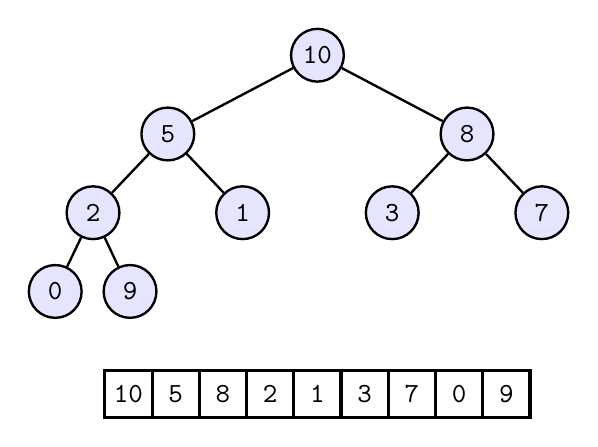
\begin{tikzpicture}

\fill[blue!10] (0.0, 0.0) circle (0.35);
\node [line width=0.03cm,black,minimum size=0.6699999999999999cm,draw,circle] at (0.0,0.0)(10){};\draw (0.0, 0.0) node[color=black] {\texttt{10}};
\fill[blue!10] (-1.9, -1.0) circle (0.35);
\node [line width=0.03cm,black,minimum size=0.6699999999999999cm,draw,circle] at (-1.9,-1.0)(5){};\draw (-1.9, -1.0) node[color=black] {\texttt{5}};
\fill[blue!10] (1.9, -1.0) circle (0.35);
\node [line width=0.03cm,black,minimum size=0.6699999999999999cm,draw,circle] at (1.9,-1.0)(8){};\draw (1.9, -1.0) node[color=black] {\texttt{8}};
\fill[blue!10] (-2.85, -2.0) circle (0.35);
\node [line width=0.03cm,black,minimum size=0.6699999999999999cm,draw,circle] at (-2.85,-2.0)(2){};\draw (-2.85, -2.0) node[color=black] {\texttt{2}};
\fill[blue!10] (-0.95, -2.0) circle (0.35);
\node [line width=0.03cm,black,minimum size=0.6699999999999999cm,draw,circle] at (-0.95,-2.0)(1){};\draw (-0.95, -2.0) node[color=black] {\texttt{1}};
\fill[blue!10] (0.95, -2.0) circle (0.35);
\node [line width=0.03cm,black,minimum size=0.6699999999999999cm,draw,circle] at (0.95,-2.0)(3){};\draw (0.95, -2.0) node[color=black] {\texttt{3}};
\fill[blue!10] (2.85, -2.0) circle (0.35);
\node [line width=0.03cm,black,minimum size=0.6699999999999999cm,draw,circle] at (2.85,-2.0)(7){};\draw (2.85, -2.0) node[color=black] {\texttt{7}};
\fill[blue!10] (-3.33, -3.0) circle (0.35);
\node [line width=0.03cm,black,minimum size=0.6699999999999999cm,draw,circle] at (-3.33,-3.0)(0){};\draw (-3.33, -3.0) node[color=black] {\texttt{0}};
\fill[blue!10] (-2.38, -3.0) circle (0.35);
\node [line width=0.03cm,black,minimum size=0.6699999999999999cm,draw,circle] at (-2.38,-3.0)(9){};\draw (-2.38, -3.0) node[color=black] {\texttt{9}};\draw[line width=0.03cm,black] (10) to  (5);
\draw[line width=0.03cm,black] (10) to  (8);
\draw[line width=0.03cm,black] (5) to  (2);
\draw[line width=0.03cm,black] (5) to  (1);
\draw[line width=0.03cm,black] (8) to  (3);
\draw[line width=0.03cm,black] (8) to  (7);
\draw[line width=0.03cm,black] (2) to  (0);
\draw[line width=0.03cm,black] (2) to  (9);

\draw (-2.3999999999999995, -4.299999999999999)
  node[draw, line width=0.04cm, , color=black,
       rounded corners=0cm, inner sep=0cm] {

\begin{minipage}[t][0.6cm]{0.6cm}
\mbox{}

\end{minipage}

};\draw (-2.3999999999999995, -4.299999999999999) node[color=black] {{\texttt{10}}};
\draw (-1.7999999999999996, -4.299999999999999)
  node[draw, line width=0.04cm, , color=black,
       rounded corners=0cm, inner sep=0cm] {

\begin{minipage}[t][0.6cm]{0.6cm}
\mbox{}

\end{minipage}

};\draw (-1.7999999999999996, -4.299999999999999) node[color=black] {{\texttt{5}}};
\draw (-1.1999999999999997, -4.299999999999999)
  node[draw, line width=0.04cm, , color=black,
       rounded corners=0cm, inner sep=0cm] {

\begin{minipage}[t][0.6cm]{0.6cm}
\mbox{}

\end{minipage}

};\draw (-1.1999999999999997, -4.299999999999999) node[color=black] {{\texttt{8}}};
\draw (-0.5999999999999996, -4.299999999999999)
  node[draw, line width=0.04cm, , color=black,
       rounded corners=0cm, inner sep=0cm] {

\begin{minipage}[t][0.6cm]{0.6cm}
\mbox{}

\end{minipage}

};\draw (-0.5999999999999996, -4.299999999999999) node[color=black] {{\texttt{2}}};
\draw (4.440892098500626e-16, -4.299999999999999)
  node[draw, line width=0.04cm, , color=black,
       rounded corners=0cm, inner sep=0cm] {

\begin{minipage}[t][0.6cm]{0.6cm}
\mbox{}

\end{minipage}

};\draw (4.440892098500626e-16, -4.299999999999999) node[color=black] {{\texttt{1}}};
\draw (0.6000000000000005, -4.299999999999999)
  node[draw, line width=0.04cm, , color=black,
       rounded corners=0cm, inner sep=0cm] {

\begin{minipage}[t][0.6cm]{0.6cm}
\mbox{}

\end{minipage}

};\draw (0.6000000000000005, -4.299999999999999) node[color=black] {{\texttt{3}}};
\draw (1.2000000000000006, -4.299999999999999)
  node[draw, line width=0.04cm, , color=black,
       rounded corners=0cm, inner sep=0cm] {

\begin{minipage}[t][0.6cm]{0.6cm}
\mbox{}

\end{minipage}

};\draw (1.2000000000000006, -4.299999999999999) node[color=black] {{\texttt{7}}};
\draw (1.8000000000000007, -4.299999999999999)
  node[draw, line width=0.04cm, , color=black,
       rounded corners=0cm, inner sep=0cm] {

\begin{minipage}[t][0.6cm]{0.6cm}
\mbox{}

\end{minipage}

};\draw (1.8000000000000007, -4.299999999999999) node[color=black] {{\texttt{0}}};
\draw (2.4000000000000004, -4.299999999999999)
  node[draw, line width=0.04cm, , color=black,
       rounded corners=0cm, inner sep=0cm] {

\begin{minipage}[t][0.6cm]{0.6cm}
\mbox{}

\end{minipage}

};\draw (2.4000000000000004, -4.299999999999999) node[color=black] {{\texttt{9}}};
\end{tikzpicture}

\end{center}



You would continue until you see the first row that is \textsc{Available}
-- this is index 0:
%-*-latex-*-

\begin{center}
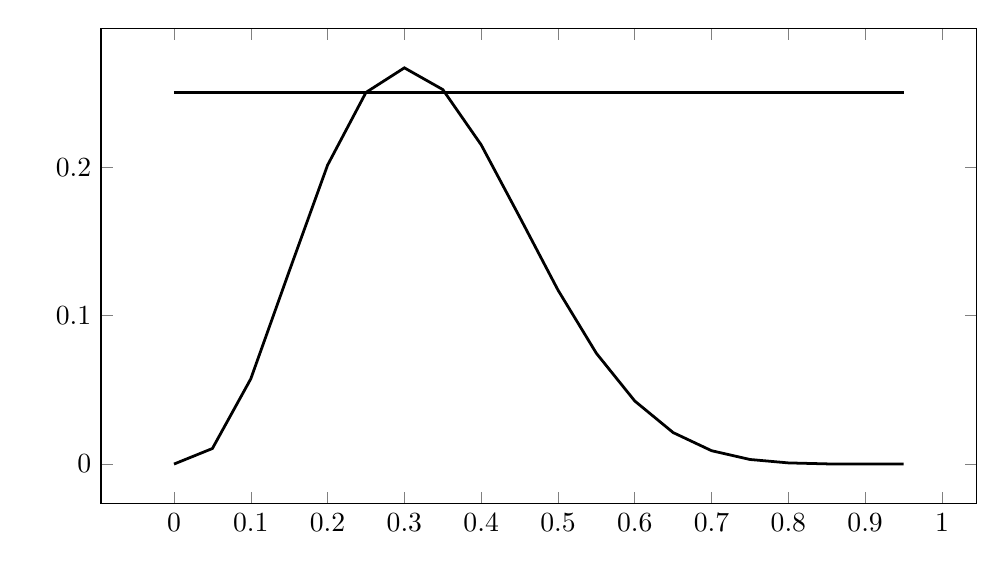
\begin{tikzpicture}[line width=1]
\begin{axis}[width=5in, height=3in,
             scatter/classes={a={mark=*,draw=black}},
             xlabel={\mbox{}},
             xlabel style={name=xlabel}, 
             ylabel={\mbox{}}, 
             legend style={
                at={(xlabel.south)},
                yshift=-1ex,
                anchor=north,
                legend cell align=left,
                },
        ]
]
\addplot[draw=black, line width=1] coordinates {(0.0, 0.0)
(0.05, 0.010475059441406248)
(0.1, 0.05739562800000002)
(0.15, 0.1298337207539062)
(0.2, 0.2013265920000001)
(0.25, 0.25028228759765625)
(0.3, 0.2668279319999998)
(0.35, 0.25221962497265626)
(0.4, 0.21499084799999998)
(0.45, 0.1664782928789064)
(0.5, 0.1171875)
(0.55, 0.07460310631640622)
(0.6, 0.042467328000000006)
(0.65, 0.02120301528515624)
(0.7, 0.009001692000000007)
(0.75, 0.00308990478515625)
(0.8, 0.000786431999999999)
(0.85, 0.0001259148164062501)
(0.9, 8.747999999999988e-06)
(0.95, 8.037890625000049e-08)};\addplot[draw=black, line width=1] coordinates {(0.0, 0.25)
(0.05, 0.25)
(0.1, 0.25)
(0.15, 0.25)
(0.2, 0.25)
(0.25, 0.25)
(0.3, 0.25)
(0.35, 0.25)
(0.4, 0.25)
(0.45, 0.25)
(0.5, 0.25)
(0.55, 0.25)
(0.6, 0.25)
(0.65, 0.25)
(0.7, 0.25)
(0.75, 0.25)
(0.8, 0.25)
(0.85, 0.25)
(0.9, 0.25)
(0.95, 0.25)};
\end{axis}\end{tikzpicture}\end{center}


Since, up to this point in time, you have not seen Toby, you know
that you can safely add (Toby, 6.3) at index 7 and mark that row
as \textsc{Not-Available}:
%-*-latex-*-

\begin{center}
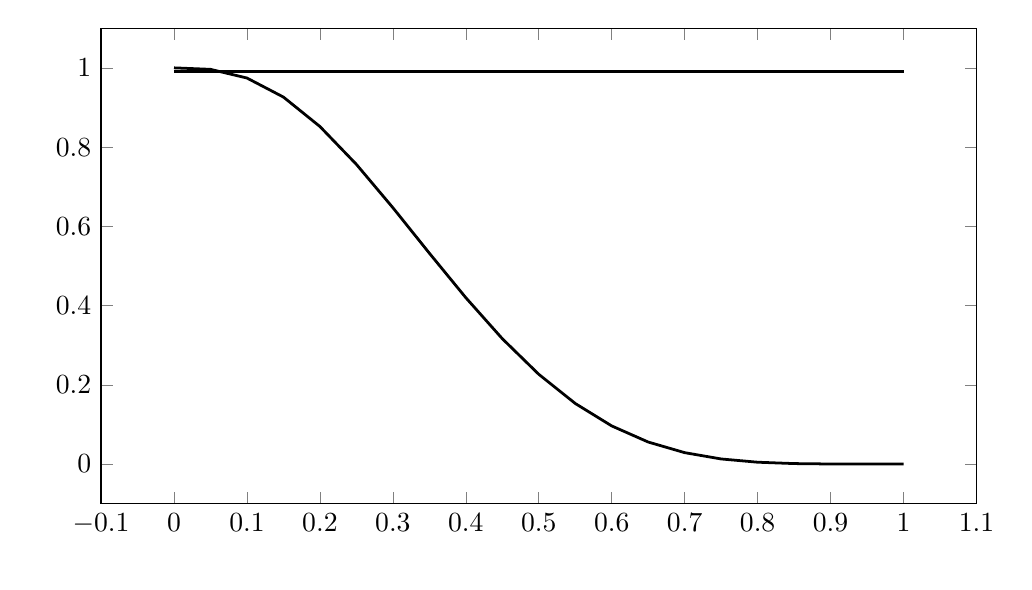
\begin{tikzpicture}[line width=1]
\begin{axis}[width=5in, height=3in,
             scatter/classes={a={mark=*,draw=black}},
             xlabel={\mbox{}},
             xlabel style={name=xlabel}, 
             ylabel={\mbox{}}, 
             legend style={
                at={(xlabel.south)},
                yshift=-1ex,
                anchor=north,
                legend cell align=left,
                },
        ]
]
\addplot[draw=black, line width=1] coordinates {(0.0, 1.0)
(0.05, 0.9962429570312497)
(0.1, 0.9743085000000002)
(0.15, 0.9262348398437498)
(0.2, 0.8519680000000004)
(0.25, 0.75640869140625)
(0.3, 0.6470694999999997)
(0.35, 0.53228332421875)
(0.4, 0.41990399999999994)
(0.45, 0.31644005078125015)
(0.5, 0.2265625)
(0.55, 0.15292768359374995)
(0.6, 0.09625600000000004)
(0.65, 0.055607535156249985)
(0.7, 0.02879550000000002)
(0.75, 0.01287841796875)
(0.8, 0.004671999999999996)
(0.85, 0.0012216445312500006)
(0.9, 0.00017649999999999982)
(0.95, 6.0273437500000275e-06)
(1.0, 0.0)};\addplot[draw=black, line width=1] coordinates {(0.0, 0.99)
(0.05, 0.99)
(0.1, 0.99)
(0.15, 0.99)
(0.2, 0.99)
(0.25, 0.99)
(0.3, 0.99)
(0.35, 0.99)
(0.4, 0.99)
(0.45, 0.99)
(0.5, 0.99)
(0.55, 0.99)
(0.6, 0.99)
(0.65, 0.99)
(0.7, 0.99)
(0.75, 0.99)
(0.8, 0.99)
(0.85, 0.99)
(0.9, 0.99)
(0.95, 0.99)
(1.0, 0.99)};
\end{axis}\end{tikzpicture}\end{center}


For delete, this is like search.
When the key is found, we mark the row as \textsc{Deleted}.



\begin{Verbatim}[frame=single]
ALGORITHM: HASHTABLE-INSERT
INPUT: hashtable of size n
       hash - hash function
       (key, value) - keyvalue pair to insert

index = -1
compute h = hash(key) % n
while 1:
    if hashtable[h].flag is DELETED:
        index = h
    else if hashtable[h].flag is AVAILABLE:
        if index == -1:
            index = h
        put (key, value) at hashtable[h] and mark that
        row as not available
        return SUCCESS
    else if hashtable[h].flag is NOT-AVAILABLE:
        if hashtable[h].key == key:
            return ERROR (i.e. key already exists)
    
    apply your probing method to compute the next h value
    if h is a previous h value:
        return ERROR
\end{Verbatim}

\begin{Verbatim}[frame=single]
ALGORITHM: HASHTABLE-DELETE
INPUT: hashtable of size n
       key

deleted = false
compute h = hash(key) % n

while 1:
    
    if hashtable[h].flag is NOT-AVAILABLE:
        if hashtable[h].key is key:
            hashtable[h].flag = DELETED
            return SUCCESS
    else if hashtable[h].flag is AVAILABLE:
        return FAILURE (i.e. key is not found)

    else:
        do nothing

    apply your probing method to compute the next h value
    if h is a previous h value:
        return FAILURE
\end{Verbatim}


\begin{console}
ALGORITHM: HASHTABLE-FIND
INPUT: hashtable of size n
       key
OUTPUT: index i where hashtable[h].key is key
            -1 is returned is key is not found

compute h = hash(key) % n

while 1:

    if hashtable[h].flag is AVAILABLE:
        return -1 (i.e., key not found)

    else if hashtable[h].flag is NOT-AVAILABLE:
        if hashtable[h].key is key:
            return h
            
    else:
        do nothing
        
    apply your probing method to compute the next h value
    if h is a previous h value:
        return FAILURE
\end{console}
(Of course you can also have a find operation that returns a pointer
to the relevant row in the table.)

Note that there's since we are marking rows as \textsc{Deleted},
a possible useful operation is to find a row that was deleted
and undelete that row -- if it has not been already overwritten
by an insert operation.


\begin{ex} 
  \label{ex:some-decision1}
  \tinysidebar{\debug{exercises/{empty0/question.tex}}}
  \solutionlink{sol:some-decision1}
  \qed
\end{ex} 
\begin{python0}
from solutions import *
add(label="ex:some-decision1",
    srcfilename='exercises/some-decision1/answer.tex') 
\end{python0}


Use this table:
\begin{center}
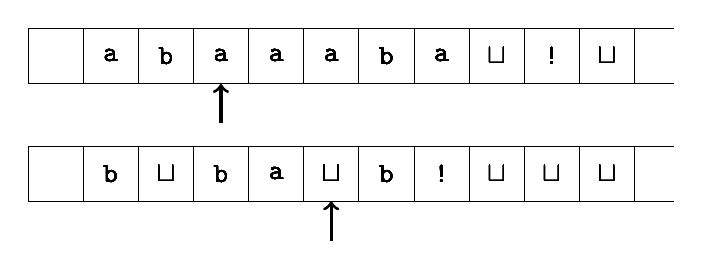
\begin{tikzpicture}

\draw (0.35, 0.35)
  node[draw, line width=0.01cm, , color=black,
       rounded corners=0cm, inner sep=0cm] {

\begin{minipage}[t][0.7cm]{0.7cm}
\mbox{}

\end{minipage}

};\draw (0.35, 0.35) node[color=black] {\texttt{\DOLLAR}};
\draw (1.0499999999999998, 0.35)
  node[draw, line width=0.01cm, , color=black,
       rounded corners=0cm, inner sep=0cm] {

\begin{minipage}[t][0.7cm]{0.7cm}
\mbox{}

\end{minipage}

};\draw (1.0499999999999998, 0.35) node[color=black] {\texttt{a}};
\draw (1.7499999999999998, 0.35)
  node[draw, line width=0.01cm, , color=black,
       rounded corners=0cm, inner sep=0cm] {

\begin{minipage}[t][0.7cm]{0.7cm}
\mbox{}

\end{minipage}

};\draw (1.7499999999999998, 0.35) node[color=black] {\texttt{b}};
\draw (2.4499999999999997, 0.35)
  node[draw, line width=0.01cm, , color=black,
       rounded corners=0cm, inner sep=0cm] {

\begin{minipage}[t][0.7cm]{0.7cm}
\mbox{}

\end{minipage}

};\draw (2.4499999999999997, 0.35) node[color=black] {\texttt{a}};
\draw (3.15, 0.35)
  node[draw, line width=0.01cm, , color=black,
       rounded corners=0cm, inner sep=0cm] {

\begin{minipage}[t][0.7cm]{0.7cm}
\mbox{}

\end{minipage}

};\draw (3.15, 0.35) node[color=black] {\texttt{a}};
\draw (3.85, 0.35)
  node[draw, line width=0.01cm, , color=black,
       rounded corners=0cm, inner sep=0cm] {

\begin{minipage}[t][0.7cm]{0.7cm}
\mbox{}

\end{minipage}

};\draw (3.85, 0.35) node[color=black] {\texttt{a}};
\draw (4.550000000000001, 0.35)
  node[draw, line width=0.01cm, , color=black,
       rounded corners=0cm, inner sep=0cm] {

\begin{minipage}[t][0.7cm]{0.7cm}
\mbox{}

\end{minipage}

};\draw (4.550000000000001, 0.35) node[color=black] {\texttt{b}};
\draw (5.25, 0.35)
  node[draw, line width=0.01cm, , color=black,
       rounded corners=0cm, inner sep=0cm] {

\begin{minipage}[t][0.7cm]{0.7cm}
\mbox{}

\end{minipage}

};\draw (5.25, 0.35) node[color=black] {\texttt{a}};
\draw (5.950000000000001, 0.35)
  node[draw, line width=0.01cm, , color=black,
       rounded corners=0cm, inner sep=0cm] {

\begin{minipage}[t][0.7cm]{0.7cm}
\mbox{}

\end{minipage}

};\draw (5.950000000000001, 0.35) node[color=black] {\texttt{$\sqcup$}};
\draw (6.65, 0.35)
  node[draw, line width=0.01cm, , color=black,
       rounded corners=0cm, inner sep=0cm] {

\begin{minipage}[t][0.7cm]{0.7cm}
\mbox{}

\end{minipage}

};\draw (6.65, 0.35) node[color=black] {\texttt{!}};
\draw (7.350000000000001, 0.35)
  node[draw, line width=0.01cm, , color=black,
       rounded corners=0cm, inner sep=0cm] {

\begin{minipage}[t][0.7cm]{0.7cm}
\mbox{}

\end{minipage}

};\draw (7.350000000000001, 0.35) node[color=black] {\texttt{$\sqcup$}};
\draw (0.35, 0.35)
  node[draw, line width=0.01cm, , color=black,
       rounded corners=0cm, inner sep=0cm] {

\begin{minipage}[t][0.7cm]{0.7cm}
\mbox{}

\end{minipage}

};\draw (0.35, 0.35) node[color=black] {\texttt{\DOLLAR}};
\draw (1.0499999999999998, 0.35)
  node[draw, line width=0.01cm, , color=black,
       rounded corners=0cm, inner sep=0cm] {

\begin{minipage}[t][0.7cm]{0.7cm}
\mbox{}

\end{minipage}

};\draw (1.0499999999999998, 0.35) node[color=black] {\texttt{a}};
\draw (1.7499999999999998, 0.35)
  node[draw, line width=0.01cm, , color=black,
       rounded corners=0cm, inner sep=0cm] {

\begin{minipage}[t][0.7cm]{0.7cm}
\mbox{}

\end{minipage}

};\draw (1.7499999999999998, 0.35) node[color=black] {\texttt{b}};
\draw (2.4499999999999997, 0.35)
  node[draw, line width=0.01cm, , color=black,
       rounded corners=0cm, inner sep=0cm] {

\begin{minipage}[t][0.7cm]{0.7cm}
\mbox{}

\end{minipage}

};\draw (2.4499999999999997, 0.35) node[color=black] {\texttt{a}};
\draw (3.15, 0.35)
  node[draw, line width=0.01cm, , color=black,
       rounded corners=0cm, inner sep=0cm] {

\begin{minipage}[t][0.7cm]{0.7cm}
\mbox{}

\end{minipage}

};\draw (3.15, 0.35) node[color=black] {\texttt{a}};
\draw (3.85, 0.35)
  node[draw, line width=0.01cm, , color=black,
       rounded corners=0cm, inner sep=0cm] {

\begin{minipage}[t][0.7cm]{0.7cm}
\mbox{}

\end{minipage}

};\draw (3.85, 0.35) node[color=black] {\texttt{a}};
\draw (4.550000000000001, 0.35)
  node[draw, line width=0.01cm, , color=black,
       rounded corners=0cm, inner sep=0cm] {

\begin{minipage}[t][0.7cm]{0.7cm}
\mbox{}

\end{minipage}

};\draw (4.550000000000001, 0.35) node[color=black] {\texttt{b}};
\draw (5.25, 0.35)
  node[draw, line width=0.01cm, , color=black,
       rounded corners=0cm, inner sep=0cm] {

\begin{minipage}[t][0.7cm]{0.7cm}
\mbox{}

\end{minipage}

};\draw (5.25, 0.35) node[color=black] {\texttt{a}};
\draw (5.950000000000001, 0.35)
  node[draw, line width=0.01cm, , color=black,
       rounded corners=0cm, inner sep=0cm] {

\begin{minipage}[t][0.7cm]{0.7cm}
\mbox{}

\end{minipage}

};\draw (5.950000000000001, 0.35) node[color=black] {\texttt{$\sqcup$}};
\draw (6.65, 0.35)
  node[draw, line width=0.01cm, , color=black,
       rounded corners=0cm, inner sep=0cm] {

\begin{minipage}[t][0.7cm]{0.7cm}
\mbox{}

\end{minipage}

};\draw (6.65, 0.35) node[color=black] {\texttt{!}};
\draw (7.350000000000001, 0.35)
  node[draw, line width=0.01cm, , color=black,
       rounded corners=0cm, inner sep=0cm] {

\begin{minipage}[t][0.7cm]{0.7cm}
\mbox{}

\end{minipage}

};\draw (7.350000000000001, 0.35) node[color=black] {\texttt{$\sqcup$}};
\draw (0.35, 0.35)
  node[draw, line width=0.01cm, , color=black,
       rounded corners=0cm, inner sep=0cm] {

\begin{minipage}[t][0.7cm]{0.7cm}
\mbox{}

\end{minipage}

};\draw (0.35, 0.35) node[color=black] {\texttt{\DOLLAR}};
\draw (1.0499999999999998, 0.35)
  node[draw, line width=0.01cm, , color=black,
       rounded corners=0cm, inner sep=0cm] {

\begin{minipage}[t][0.7cm]{0.7cm}
\mbox{}

\end{minipage}

};\draw (1.0499999999999998, 0.35) node[color=black] {\texttt{a}};
\draw (1.7499999999999998, 0.35)
  node[draw, line width=0.01cm, , color=black,
       rounded corners=0cm, inner sep=0cm] {

\begin{minipage}[t][0.7cm]{0.7cm}
\mbox{}

\end{minipage}

};\draw (1.7499999999999998, 0.35) node[color=black] {\texttt{b}};
\draw (2.4499999999999997, 0.35)
  node[draw, line width=0.01cm, , color=black,
       rounded corners=0cm, inner sep=0cm] {

\begin{minipage}[t][0.7cm]{0.7cm}
\mbox{}

\end{minipage}

};\draw (2.4499999999999997, 0.35) node[color=black] {\texttt{a}};
\draw (3.15, 0.35)
  node[draw, line width=0.01cm, , color=black,
       rounded corners=0cm, inner sep=0cm] {

\begin{minipage}[t][0.7cm]{0.7cm}
\mbox{}

\end{minipage}

};\draw (3.15, 0.35) node[color=black] {\texttt{a}};
\draw (3.85, 0.35)
  node[draw, line width=0.01cm, , color=black,
       rounded corners=0cm, inner sep=0cm] {

\begin{minipage}[t][0.7cm]{0.7cm}
\mbox{}

\end{minipage}

};\draw (3.85, 0.35) node[color=black] {\texttt{a}};
\draw (4.550000000000001, 0.35)
  node[draw, line width=0.01cm, , color=black,
       rounded corners=0cm, inner sep=0cm] {

\begin{minipage}[t][0.7cm]{0.7cm}
\mbox{}

\end{minipage}

};\draw (4.550000000000001, 0.35) node[color=black] {\texttt{b}};
\draw (5.25, 0.35)
  node[draw, line width=0.01cm, , color=black,
       rounded corners=0cm, inner sep=0cm] {

\begin{minipage}[t][0.7cm]{0.7cm}
\mbox{}

\end{minipage}

};\draw (5.25, 0.35) node[color=black] {\texttt{a}};
\draw (5.950000000000001, 0.35)
  node[draw, line width=0.01cm, , color=black,
       rounded corners=0cm, inner sep=0cm] {

\begin{minipage}[t][0.7cm]{0.7cm}
\mbox{}

\end{minipage}

};\draw (5.950000000000001, 0.35) node[color=black] {\texttt{$\sqcup$}};
\draw (6.65, 0.35)
  node[draw, line width=0.01cm, , color=black,
       rounded corners=0cm, inner sep=0cm] {

\begin{minipage}[t][0.7cm]{0.7cm}
\mbox{}

\end{minipage}

};\draw (6.65, 0.35) node[color=black] {\texttt{!}};
\draw (7.350000000000001, 0.35)
  node[draw, line width=0.01cm, , color=black,
       rounded corners=0cm, inner sep=0cm] {

\begin{minipage}[t][0.7cm]{0.7cm}
\mbox{}

\end{minipage}

};\draw (7.350000000000001, 0.35) node[color=black] {\texttt{$\sqcup$}};
\draw (0.35, 0.35)
  node[draw, line width=0.01cm, , color=black,
       rounded corners=0cm, inner sep=0cm] {

\begin{minipage}[t][0.7cm]{0.7cm}
\mbox{}

\end{minipage}

};\draw (0.35, 0.35) node[color=black] {\texttt{\DOLLAR}};
\draw (1.0499999999999998, 0.35)
  node[draw, line width=0.01cm, , color=black,
       rounded corners=0cm, inner sep=0cm] {

\begin{minipage}[t][0.7cm]{0.7cm}
\mbox{}

\end{minipage}

};\draw (1.0499999999999998, 0.35) node[color=black] {\texttt{a}};
\draw (1.7499999999999998, 0.35)
  node[draw, line width=0.01cm, , color=black,
       rounded corners=0cm, inner sep=0cm] {

\begin{minipage}[t][0.7cm]{0.7cm}
\mbox{}

\end{minipage}

};\draw (1.7499999999999998, 0.35) node[color=black] {\texttt{b}};
\draw (2.4499999999999997, 0.35)
  node[draw, line width=0.01cm, , color=black,
       rounded corners=0cm, inner sep=0cm] {

\begin{minipage}[t][0.7cm]{0.7cm}
\mbox{}

\end{minipage}

};\draw (2.4499999999999997, 0.35) node[color=black] {\texttt{a}};
\draw (3.15, 0.35)
  node[draw, line width=0.01cm, , color=black,
       rounded corners=0cm, inner sep=0cm] {

\begin{minipage}[t][0.7cm]{0.7cm}
\mbox{}

\end{minipage}

};\draw (3.15, 0.35) node[color=black] {\texttt{a}};
\draw (3.85, 0.35)
  node[draw, line width=0.01cm, , color=black,
       rounded corners=0cm, inner sep=0cm] {

\begin{minipage}[t][0.7cm]{0.7cm}
\mbox{}

\end{minipage}

};\draw (3.85, 0.35) node[color=black] {\texttt{a}};
\draw (4.550000000000001, 0.35)
  node[draw, line width=0.01cm, , color=black,
       rounded corners=0cm, inner sep=0cm] {

\begin{minipage}[t][0.7cm]{0.7cm}
\mbox{}

\end{minipage}

};\draw (4.550000000000001, 0.35) node[color=black] {\texttt{b}};
\draw (5.25, 0.35)
  node[draw, line width=0.01cm, , color=black,
       rounded corners=0cm, inner sep=0cm] {

\begin{minipage}[t][0.7cm]{0.7cm}
\mbox{}

\end{minipage}

};\draw (5.25, 0.35) node[color=black] {\texttt{a}};
\draw (5.950000000000001, 0.35)
  node[draw, line width=0.01cm, , color=black,
       rounded corners=0cm, inner sep=0cm] {

\begin{minipage}[t][0.7cm]{0.7cm}
\mbox{}

\end{minipage}

};\draw (5.950000000000001, 0.35) node[color=black] {\texttt{$\sqcup$}};
\draw (6.65, 0.35)
  node[draw, line width=0.01cm, , color=black,
       rounded corners=0cm, inner sep=0cm] {

\begin{minipage}[t][0.7cm]{0.7cm}
\mbox{}

\end{minipage}

};\draw (6.65, 0.35) node[color=black] {\texttt{!}};
\draw (7.350000000000001, 0.35)
  node[draw, line width=0.01cm, , color=black,
       rounded corners=0cm, inner sep=0cm] {

\begin{minipage}[t][0.7cm]{0.7cm}
\mbox{}

\end{minipage}

};\draw (7.350000000000001, 0.35) node[color=black] {\texttt{$\sqcup$}};
\draw (0.35, 0.35)
  node[draw, line width=0.01cm, , color=black,
       rounded corners=0cm, inner sep=0cm] {

\begin{minipage}[t][0.7cm]{0.7cm}
\mbox{}

\end{minipage}

};\draw (0.35, 0.35) node[color=black] {\texttt{\DOLLAR}};
\draw (1.0499999999999998, 0.35)
  node[draw, line width=0.01cm, , color=black,
       rounded corners=0cm, inner sep=0cm] {

\begin{minipage}[t][0.7cm]{0.7cm}
\mbox{}

\end{minipage}

};\draw (1.0499999999999998, 0.35) node[color=black] {\texttt{a}};
\draw (1.7499999999999998, 0.35)
  node[draw, line width=0.01cm, , color=black,
       rounded corners=0cm, inner sep=0cm] {

\begin{minipage}[t][0.7cm]{0.7cm}
\mbox{}

\end{minipage}

};\draw (1.7499999999999998, 0.35) node[color=black] {\texttt{b}};
\draw (2.4499999999999997, 0.35)
  node[draw, line width=0.01cm, , color=black,
       rounded corners=0cm, inner sep=0cm] {

\begin{minipage}[t][0.7cm]{0.7cm}
\mbox{}

\end{minipage}

};\draw (2.4499999999999997, 0.35) node[color=black] {\texttt{a}};
\draw (3.15, 0.35)
  node[draw, line width=0.01cm, , color=black,
       rounded corners=0cm, inner sep=0cm] {

\begin{minipage}[t][0.7cm]{0.7cm}
\mbox{}

\end{minipage}

};\draw (3.15, 0.35) node[color=black] {\texttt{a}};
\draw (3.85, 0.35)
  node[draw, line width=0.01cm, , color=black,
       rounded corners=0cm, inner sep=0cm] {

\begin{minipage}[t][0.7cm]{0.7cm}
\mbox{}

\end{minipage}

};\draw (3.85, 0.35) node[color=black] {\texttt{a}};
\draw (4.550000000000001, 0.35)
  node[draw, line width=0.01cm, , color=black,
       rounded corners=0cm, inner sep=0cm] {

\begin{minipage}[t][0.7cm]{0.7cm}
\mbox{}

\end{minipage}

};\draw (4.550000000000001, 0.35) node[color=black] {\texttt{b}};
\draw (5.25, 0.35)
  node[draw, line width=0.01cm, , color=black,
       rounded corners=0cm, inner sep=0cm] {

\begin{minipage}[t][0.7cm]{0.7cm}
\mbox{}

\end{minipage}

};\draw (5.25, 0.35) node[color=black] {\texttt{a}};
\draw (5.950000000000001, 0.35)
  node[draw, line width=0.01cm, , color=black,
       rounded corners=0cm, inner sep=0cm] {

\begin{minipage}[t][0.7cm]{0.7cm}
\mbox{}

\end{minipage}

};\draw (5.950000000000001, 0.35) node[color=black] {\texttt{$\sqcup$}};
\draw (6.65, 0.35)
  node[draw, line width=0.01cm, , color=black,
       rounded corners=0cm, inner sep=0cm] {

\begin{minipage}[t][0.7cm]{0.7cm}
\mbox{}

\end{minipage}

};\draw (6.65, 0.35) node[color=black] {\texttt{!}};
\draw (7.350000000000001, 0.35)
  node[draw, line width=0.01cm, , color=black,
       rounded corners=0cm, inner sep=0cm] {

\begin{minipage}[t][0.7cm]{0.7cm}
\mbox{}

\end{minipage}

};\draw (7.350000000000001, 0.35) node[color=black] {\texttt{$\sqcup$}};
\draw (0.35, 0.35)
  node[draw, line width=0.01cm, , color=black,
       rounded corners=0cm, inner sep=0cm] {

\begin{minipage}[t][0.7cm]{0.7cm}
\mbox{}

\end{minipage}

};\draw (0.35, 0.35) node[color=black] {\texttt{\DOLLAR}};
\draw (1.0499999999999998, 0.35)
  node[draw, line width=0.01cm, , color=black,
       rounded corners=0cm, inner sep=0cm] {

\begin{minipage}[t][0.7cm]{0.7cm}
\mbox{}

\end{minipage}

};\draw (1.0499999999999998, 0.35) node[color=black] {\texttt{a}};
\draw (1.7499999999999998, 0.35)
  node[draw, line width=0.01cm, , color=black,
       rounded corners=0cm, inner sep=0cm] {

\begin{minipage}[t][0.7cm]{0.7cm}
\mbox{}

\end{minipage}

};\draw (1.7499999999999998, 0.35) node[color=black] {\texttt{b}};
\draw (2.4499999999999997, 0.35)
  node[draw, line width=0.01cm, , color=black,
       rounded corners=0cm, inner sep=0cm] {

\begin{minipage}[t][0.7cm]{0.7cm}
\mbox{}

\end{minipage}

};\draw (2.4499999999999997, 0.35) node[color=black] {\texttt{a}};
\draw (3.15, 0.35)
  node[draw, line width=0.01cm, , color=black,
       rounded corners=0cm, inner sep=0cm] {

\begin{minipage}[t][0.7cm]{0.7cm}
\mbox{}

\end{minipage}

};\draw (3.15, 0.35) node[color=black] {\texttt{a}};
\draw (3.85, 0.35)
  node[draw, line width=0.01cm, , color=black,
       rounded corners=0cm, inner sep=0cm] {

\begin{minipage}[t][0.7cm]{0.7cm}
\mbox{}

\end{minipage}

};\draw (3.85, 0.35) node[color=black] {\texttt{a}};
\draw (4.550000000000001, 0.35)
  node[draw, line width=0.01cm, , color=black,
       rounded corners=0cm, inner sep=0cm] {

\begin{minipage}[t][0.7cm]{0.7cm}
\mbox{}

\end{minipage}

};\draw (4.550000000000001, 0.35) node[color=black] {\texttt{b}};
\draw (5.25, 0.35)
  node[draw, line width=0.01cm, , color=black,
       rounded corners=0cm, inner sep=0cm] {

\begin{minipage}[t][0.7cm]{0.7cm}
\mbox{}

\end{minipage}

};\draw (5.25, 0.35) node[color=black] {\texttt{a}};
\draw (5.950000000000001, 0.35)
  node[draw, line width=0.01cm, , color=black,
       rounded corners=0cm, inner sep=0cm] {

\begin{minipage}[t][0.7cm]{0.7cm}
\mbox{}

\end{minipage}

};\draw (5.950000000000001, 0.35) node[color=black] {\texttt{$\sqcup$}};
\draw (6.65, 0.35)
  node[draw, line width=0.01cm, , color=black,
       rounded corners=0cm, inner sep=0cm] {

\begin{minipage}[t][0.7cm]{0.7cm}
\mbox{}

\end{minipage}

};\draw (6.65, 0.35) node[color=black] {\texttt{!}};
\draw (7.350000000000001, 0.35)
  node[draw, line width=0.01cm, , color=black,
       rounded corners=0cm, inner sep=0cm] {

\begin{minipage}[t][0.7cm]{0.7cm}
\mbox{}

\end{minipage}

};\draw (7.350000000000001, 0.35) node[color=black] {\texttt{$\sqcup$}};
\draw (0.35, 0.35)
  node[draw, line width=0.01cm, , color=black,
       rounded corners=0cm, inner sep=0cm] {

\begin{minipage}[t][0.7cm]{0.7cm}
\mbox{}

\end{minipage}

};\draw (0.35, 0.35) node[color=black] {\texttt{\DOLLAR}};
\draw (1.0499999999999998, 0.35)
  node[draw, line width=0.01cm, , color=black,
       rounded corners=0cm, inner sep=0cm] {

\begin{minipage}[t][0.7cm]{0.7cm}
\mbox{}

\end{minipage}

};\draw (1.0499999999999998, 0.35) node[color=black] {\texttt{a}};
\draw (1.7499999999999998, 0.35)
  node[draw, line width=0.01cm, , color=black,
       rounded corners=0cm, inner sep=0cm] {

\begin{minipage}[t][0.7cm]{0.7cm}
\mbox{}

\end{minipage}

};\draw (1.7499999999999998, 0.35) node[color=black] {\texttt{b}};
\draw (2.4499999999999997, 0.35)
  node[draw, line width=0.01cm, , color=black,
       rounded corners=0cm, inner sep=0cm] {

\begin{minipage}[t][0.7cm]{0.7cm}
\mbox{}

\end{minipage}

};\draw (2.4499999999999997, 0.35) node[color=black] {\texttt{a}};
\draw (3.15, 0.35)
  node[draw, line width=0.01cm, , color=black,
       rounded corners=0cm, inner sep=0cm] {

\begin{minipage}[t][0.7cm]{0.7cm}
\mbox{}

\end{minipage}

};\draw (3.15, 0.35) node[color=black] {\texttt{a}};
\draw (3.85, 0.35)
  node[draw, line width=0.01cm, , color=black,
       rounded corners=0cm, inner sep=0cm] {

\begin{minipage}[t][0.7cm]{0.7cm}
\mbox{}

\end{minipage}

};\draw (3.85, 0.35) node[color=black] {\texttt{a}};
\draw (4.550000000000001, 0.35)
  node[draw, line width=0.01cm, , color=black,
       rounded corners=0cm, inner sep=0cm] {

\begin{minipage}[t][0.7cm]{0.7cm}
\mbox{}

\end{minipage}

};\draw (4.550000000000001, 0.35) node[color=black] {\texttt{b}};
\draw (5.25, 0.35)
  node[draw, line width=0.01cm, , color=black,
       rounded corners=0cm, inner sep=0cm] {

\begin{minipage}[t][0.7cm]{0.7cm}
\mbox{}

\end{minipage}

};\draw (5.25, 0.35) node[color=black] {\texttt{a}};
\draw (5.950000000000001, 0.35)
  node[draw, line width=0.01cm, , color=black,
       rounded corners=0cm, inner sep=0cm] {

\begin{minipage}[t][0.7cm]{0.7cm}
\mbox{}

\end{minipage}

};\draw (5.950000000000001, 0.35) node[color=black] {\texttt{$\sqcup$}};
\draw (6.65, 0.35)
  node[draw, line width=0.01cm, , color=black,
       rounded corners=0cm, inner sep=0cm] {

\begin{minipage}[t][0.7cm]{0.7cm}
\mbox{}

\end{minipage}

};\draw (6.65, 0.35) node[color=black] {\texttt{!}};
\draw (7.350000000000001, 0.35)
  node[draw, line width=0.01cm, , color=black,
       rounded corners=0cm, inner sep=0cm] {

\begin{minipage}[t][0.7cm]{0.7cm}
\mbox{}

\end{minipage}

};\draw (7.350000000000001, 0.35) node[color=black] {\texttt{$\sqcup$}};
\draw (0.35, 0.35)
  node[draw, line width=0.01cm, , color=black,
       rounded corners=0cm, inner sep=0cm] {

\begin{minipage}[t][0.7cm]{0.7cm}
\mbox{}

\end{minipage}

};\draw (0.35, 0.35) node[color=black] {\texttt{\DOLLAR}};
\draw (1.0499999999999998, 0.35)
  node[draw, line width=0.01cm, , color=black,
       rounded corners=0cm, inner sep=0cm] {

\begin{minipage}[t][0.7cm]{0.7cm}
\mbox{}

\end{minipage}

};\draw (1.0499999999999998, 0.35) node[color=black] {\texttt{a}};
\draw (1.7499999999999998, 0.35)
  node[draw, line width=0.01cm, , color=black,
       rounded corners=0cm, inner sep=0cm] {

\begin{minipage}[t][0.7cm]{0.7cm}
\mbox{}

\end{minipage}

};\draw (1.7499999999999998, 0.35) node[color=black] {\texttt{b}};
\draw (2.4499999999999997, 0.35)
  node[draw, line width=0.01cm, , color=black,
       rounded corners=0cm, inner sep=0cm] {

\begin{minipage}[t][0.7cm]{0.7cm}
\mbox{}

\end{minipage}

};\draw (2.4499999999999997, 0.35) node[color=black] {\texttt{a}};
\draw (3.15, 0.35)
  node[draw, line width=0.01cm, , color=black,
       rounded corners=0cm, inner sep=0cm] {

\begin{minipage}[t][0.7cm]{0.7cm}
\mbox{}

\end{minipage}

};\draw (3.15, 0.35) node[color=black] {\texttt{a}};
\draw (3.85, 0.35)
  node[draw, line width=0.01cm, , color=black,
       rounded corners=0cm, inner sep=0cm] {

\begin{minipage}[t][0.7cm]{0.7cm}
\mbox{}

\end{minipage}

};\draw (3.85, 0.35) node[color=black] {\texttt{a}};
\draw (4.550000000000001, 0.35)
  node[draw, line width=0.01cm, , color=black,
       rounded corners=0cm, inner sep=0cm] {

\begin{minipage}[t][0.7cm]{0.7cm}
\mbox{}

\end{minipage}

};\draw (4.550000000000001, 0.35) node[color=black] {\texttt{b}};
\draw (5.25, 0.35)
  node[draw, line width=0.01cm, , color=black,
       rounded corners=0cm, inner sep=0cm] {

\begin{minipage}[t][0.7cm]{0.7cm}
\mbox{}

\end{minipage}

};\draw (5.25, 0.35) node[color=black] {\texttt{a}};
\draw (5.950000000000001, 0.35)
  node[draw, line width=0.01cm, , color=black,
       rounded corners=0cm, inner sep=0cm] {

\begin{minipage}[t][0.7cm]{0.7cm}
\mbox{}

\end{minipage}

};\draw (5.950000000000001, 0.35) node[color=black] {\texttt{$\sqcup$}};
\draw (6.65, 0.35)
  node[draw, line width=0.01cm, , color=black,
       rounded corners=0cm, inner sep=0cm] {

\begin{minipage}[t][0.7cm]{0.7cm}
\mbox{}

\end{minipage}

};\draw (6.65, 0.35) node[color=black] {\texttt{!}};
\draw (7.350000000000001, 0.35)
  node[draw, line width=0.01cm, , color=black,
       rounded corners=0cm, inner sep=0cm] {

\begin{minipage}[t][0.7cm]{0.7cm}
\mbox{}

\end{minipage}

};\draw (7.350000000000001, 0.35) node[color=black] {\texttt{$\sqcup$}};
\draw (0.35, 0.35)
  node[draw, line width=0.01cm, , color=black,
       rounded corners=0cm, inner sep=0cm] {

\begin{minipage}[t][0.7cm]{0.7cm}
\mbox{}

\end{minipage}

};\draw (0.35, 0.35) node[color=black] {\texttt{\DOLLAR}};
\draw (1.0499999999999998, 0.35)
  node[draw, line width=0.01cm, , color=black,
       rounded corners=0cm, inner sep=0cm] {

\begin{minipage}[t][0.7cm]{0.7cm}
\mbox{}

\end{minipage}

};\draw (1.0499999999999998, 0.35) node[color=black] {\texttt{a}};
\draw (1.7499999999999998, 0.35)
  node[draw, line width=0.01cm, , color=black,
       rounded corners=0cm, inner sep=0cm] {

\begin{minipage}[t][0.7cm]{0.7cm}
\mbox{}

\end{minipage}

};\draw (1.7499999999999998, 0.35) node[color=black] {\texttt{b}};
\draw (2.4499999999999997, 0.35)
  node[draw, line width=0.01cm, , color=black,
       rounded corners=0cm, inner sep=0cm] {

\begin{minipage}[t][0.7cm]{0.7cm}
\mbox{}

\end{minipage}

};\draw (2.4499999999999997, 0.35) node[color=black] {\texttt{a}};
\draw (3.15, 0.35)
  node[draw, line width=0.01cm, , color=black,
       rounded corners=0cm, inner sep=0cm] {

\begin{minipage}[t][0.7cm]{0.7cm}
\mbox{}

\end{minipage}

};\draw (3.15, 0.35) node[color=black] {\texttt{a}};
\draw (3.85, 0.35)
  node[draw, line width=0.01cm, , color=black,
       rounded corners=0cm, inner sep=0cm] {

\begin{minipage}[t][0.7cm]{0.7cm}
\mbox{}

\end{minipage}

};\draw (3.85, 0.35) node[color=black] {\texttt{a}};
\draw (4.550000000000001, 0.35)
  node[draw, line width=0.01cm, , color=black,
       rounded corners=0cm, inner sep=0cm] {

\begin{minipage}[t][0.7cm]{0.7cm}
\mbox{}

\end{minipage}

};\draw (4.550000000000001, 0.35) node[color=black] {\texttt{b}};
\draw (5.25, 0.35)
  node[draw, line width=0.01cm, , color=black,
       rounded corners=0cm, inner sep=0cm] {

\begin{minipage}[t][0.7cm]{0.7cm}
\mbox{}

\end{minipage}

};\draw (5.25, 0.35) node[color=black] {\texttt{a}};
\draw (5.950000000000001, 0.35)
  node[draw, line width=0.01cm, , color=black,
       rounded corners=0cm, inner sep=0cm] {

\begin{minipage}[t][0.7cm]{0.7cm}
\mbox{}

\end{minipage}

};\draw (5.950000000000001, 0.35) node[color=black] {\texttt{$\sqcup$}};
\draw (6.65, 0.35)
  node[draw, line width=0.01cm, , color=black,
       rounded corners=0cm, inner sep=0cm] {

\begin{minipage}[t][0.7cm]{0.7cm}
\mbox{}

\end{minipage}

};\draw (6.65, 0.35) node[color=black] {\texttt{!}};
\draw (7.350000000000001, 0.35)
  node[draw, line width=0.01cm, , color=black,
       rounded corners=0cm, inner sep=0cm] {

\begin{minipage}[t][0.7cm]{0.7cm}
\mbox{}

\end{minipage}

};\draw (7.350000000000001, 0.35) node[color=black] {\texttt{$\sqcup$}};
\draw (0.35, 0.35)
  node[draw, line width=0.01cm, , color=black,
       rounded corners=0cm, inner sep=0cm] {

\begin{minipage}[t][0.7cm]{0.7cm}
\mbox{}

\end{minipage}

};\draw (0.35, 0.35) node[color=black] {\texttt{\DOLLAR}};
\draw (1.0499999999999998, 0.35)
  node[draw, line width=0.01cm, , color=black,
       rounded corners=0cm, inner sep=0cm] {

\begin{minipage}[t][0.7cm]{0.7cm}
\mbox{}

\end{minipage}

};\draw (1.0499999999999998, 0.35) node[color=black] {\texttt{a}};
\draw (1.7499999999999998, 0.35)
  node[draw, line width=0.01cm, , color=black,
       rounded corners=0cm, inner sep=0cm] {

\begin{minipage}[t][0.7cm]{0.7cm}
\mbox{}

\end{minipage}

};\draw (1.7499999999999998, 0.35) node[color=black] {\texttt{b}};
\draw (2.4499999999999997, 0.35)
  node[draw, line width=0.01cm, , color=black,
       rounded corners=0cm, inner sep=0cm] {

\begin{minipage}[t][0.7cm]{0.7cm}
\mbox{}

\end{minipage}

};\draw (2.4499999999999997, 0.35) node[color=black] {\texttt{a}};
\draw (3.15, 0.35)
  node[draw, line width=0.01cm, , color=black,
       rounded corners=0cm, inner sep=0cm] {

\begin{minipage}[t][0.7cm]{0.7cm}
\mbox{}

\end{minipage}

};\draw (3.15, 0.35) node[color=black] {\texttt{a}};
\draw (3.85, 0.35)
  node[draw, line width=0.01cm, , color=black,
       rounded corners=0cm, inner sep=0cm] {

\begin{minipage}[t][0.7cm]{0.7cm}
\mbox{}

\end{minipage}

};\draw (3.85, 0.35) node[color=black] {\texttt{a}};
\draw (4.550000000000001, 0.35)
  node[draw, line width=0.01cm, , color=black,
       rounded corners=0cm, inner sep=0cm] {

\begin{minipage}[t][0.7cm]{0.7cm}
\mbox{}

\end{minipage}

};\draw (4.550000000000001, 0.35) node[color=black] {\texttt{b}};
\draw (5.25, 0.35)
  node[draw, line width=0.01cm, , color=black,
       rounded corners=0cm, inner sep=0cm] {

\begin{minipage}[t][0.7cm]{0.7cm}
\mbox{}

\end{minipage}

};\draw (5.25, 0.35) node[color=black] {\texttt{a}};
\draw (5.950000000000001, 0.35)
  node[draw, line width=0.01cm, , color=black,
       rounded corners=0cm, inner sep=0cm] {

\begin{minipage}[t][0.7cm]{0.7cm}
\mbox{}

\end{minipage}

};\draw (5.950000000000001, 0.35) node[color=black] {\texttt{$\sqcup$}};
\draw (6.65, 0.35)
  node[draw, line width=0.01cm, , color=black,
       rounded corners=0cm, inner sep=0cm] {

\begin{minipage}[t][0.7cm]{0.7cm}
\mbox{}

\end{minipage}

};\draw (6.65, 0.35) node[color=black] {\texttt{!}};
\draw (7.350000000000001, 0.35)
  node[draw, line width=0.01cm, , color=black,
       rounded corners=0cm, inner sep=0cm] {

\begin{minipage}[t][0.7cm]{0.7cm}
\mbox{}

\end{minipage}

};\draw (7.350000000000001, 0.35) node[color=black] {\texttt{$\sqcup$}};
\draw (0.35, 0.35)
  node[draw, line width=0.01cm, , color=black,
       rounded corners=0cm, inner sep=0cm] {

\begin{minipage}[t][0.7cm]{0.7cm}
\mbox{}

\end{minipage}

};\draw (0.35, 0.35) node[color=black] {\texttt{\DOLLAR}};
\draw (1.0499999999999998, 0.35)
  node[draw, line width=0.01cm, , color=black,
       rounded corners=0cm, inner sep=0cm] {

\begin{minipage}[t][0.7cm]{0.7cm}
\mbox{}

\end{minipage}

};\draw (1.0499999999999998, 0.35) node[color=black] {\texttt{a}};
\draw (1.7499999999999998, 0.35)
  node[draw, line width=0.01cm, , color=black,
       rounded corners=0cm, inner sep=0cm] {

\begin{minipage}[t][0.7cm]{0.7cm}
\mbox{}

\end{minipage}

};\draw (1.7499999999999998, 0.35) node[color=black] {\texttt{b}};
\draw (2.4499999999999997, 0.35)
  node[draw, line width=0.01cm, , color=black,
       rounded corners=0cm, inner sep=0cm] {

\begin{minipage}[t][0.7cm]{0.7cm}
\mbox{}

\end{minipage}

};\draw (2.4499999999999997, 0.35) node[color=black] {\texttt{a}};
\draw (3.15, 0.35)
  node[draw, line width=0.01cm, , color=black,
       rounded corners=0cm, inner sep=0cm] {

\begin{minipage}[t][0.7cm]{0.7cm}
\mbox{}

\end{minipage}

};\draw (3.15, 0.35) node[color=black] {\texttt{a}};
\draw (3.85, 0.35)
  node[draw, line width=0.01cm, , color=black,
       rounded corners=0cm, inner sep=0cm] {

\begin{minipage}[t][0.7cm]{0.7cm}
\mbox{}

\end{minipage}

};\draw (3.85, 0.35) node[color=black] {\texttt{a}};
\draw (4.550000000000001, 0.35)
  node[draw, line width=0.01cm, , color=black,
       rounded corners=0cm, inner sep=0cm] {

\begin{minipage}[t][0.7cm]{0.7cm}
\mbox{}

\end{minipage}

};\draw (4.550000000000001, 0.35) node[color=black] {\texttt{b}};
\draw (5.25, 0.35)
  node[draw, line width=0.01cm, , color=black,
       rounded corners=0cm, inner sep=0cm] {

\begin{minipage}[t][0.7cm]{0.7cm}
\mbox{}

\end{minipage}

};\draw (5.25, 0.35) node[color=black] {\texttt{a}};
\draw (5.950000000000001, 0.35)
  node[draw, line width=0.01cm, , color=black,
       rounded corners=0cm, inner sep=0cm] {

\begin{minipage}[t][0.7cm]{0.7cm}
\mbox{}

\end{minipage}

};\draw (5.950000000000001, 0.35) node[color=black] {\texttt{$\sqcup$}};
\draw (6.65, 0.35)
  node[draw, line width=0.01cm, , color=black,
       rounded corners=0cm, inner sep=0cm] {

\begin{minipage}[t][0.7cm]{0.7cm}
\mbox{}

\end{minipage}

};\draw (6.65, 0.35) node[color=black] {\texttt{!}};
\draw (7.350000000000001, 0.35)
  node[draw, line width=0.01cm, , color=black,
       rounded corners=0cm, inner sep=0cm] {

\begin{minipage}[t][0.7cm]{0.7cm}
\mbox{}

\end{minipage}

};\draw (7.350000000000001, 0.35) node[color=black] {\texttt{$\sqcup$}};\draw[line width=0.01cm,black] (7.700000000000001,0.7) to  (8.200000000000001,0.7);
\draw[line width=0.01cm,black] (7.700000000000001,0.0) to  (8.200000000000001,0.0);
\draw[line width=0.04cm,black,->] (2.45,-0.51) to  (2.45,-0.01);

\draw (0.35, -1.15)
  node[draw, line width=0.01cm, , color=black,
       rounded corners=0cm, inner sep=0cm] {

\begin{minipage}[t][0.7cm]{0.7cm}
\mbox{}

\end{minipage}

};\draw (0.35, -1.15) node[color=black] {\texttt{\DOLLAR}};
\draw (1.0499999999999998, -1.15)
  node[draw, line width=0.01cm, , color=black,
       rounded corners=0cm, inner sep=0cm] {

\begin{minipage}[t][0.7cm]{0.7cm}
\mbox{}

\end{minipage}

};\draw (1.0499999999999998, -1.15) node[color=black] {\texttt{b}};
\draw (1.7499999999999998, -1.15)
  node[draw, line width=0.01cm, , color=black,
       rounded corners=0cm, inner sep=0cm] {

\begin{minipage}[t][0.7cm]{0.7cm}
\mbox{}

\end{minipage}

};\draw (1.7499999999999998, -1.15) node[color=black] {\texttt{$\sqcup$}};
\draw (2.4499999999999997, -1.15)
  node[draw, line width=0.01cm, , color=black,
       rounded corners=0cm, inner sep=0cm] {

\begin{minipage}[t][0.7cm]{0.7cm}
\mbox{}

\end{minipage}

};\draw (2.4499999999999997, -1.15) node[color=black] {\texttt{b}};
\draw (3.15, -1.15)
  node[draw, line width=0.01cm, , color=black,
       rounded corners=0cm, inner sep=0cm] {

\begin{minipage}[t][0.7cm]{0.7cm}
\mbox{}

\end{minipage}

};\draw (3.15, -1.15) node[color=black] {\texttt{a}};
\draw (3.85, -1.15)
  node[draw, line width=0.01cm, , color=black,
       rounded corners=0cm, inner sep=0cm] {

\begin{minipage}[t][0.7cm]{0.7cm}
\mbox{}

\end{minipage}

};\draw (3.85, -1.15) node[color=black] {\texttt{$\sqcup$}};
\draw (4.550000000000001, -1.15)
  node[draw, line width=0.01cm, , color=black,
       rounded corners=0cm, inner sep=0cm] {

\begin{minipage}[t][0.7cm]{0.7cm}
\mbox{}

\end{minipage}

};\draw (4.550000000000001, -1.15) node[color=black] {\texttt{b}};
\draw (5.25, -1.15)
  node[draw, line width=0.01cm, , color=black,
       rounded corners=0cm, inner sep=0cm] {

\begin{minipage}[t][0.7cm]{0.7cm}
\mbox{}

\end{minipage}

};\draw (5.25, -1.15) node[color=black] {\texttt{!}};
\draw (5.950000000000001, -1.15)
  node[draw, line width=0.01cm, , color=black,
       rounded corners=0cm, inner sep=0cm] {

\begin{minipage}[t][0.7cm]{0.7cm}
\mbox{}

\end{minipage}

};\draw (5.950000000000001, -1.15) node[color=black] {\texttt{$\sqcup$}};
\draw (6.65, -1.15)
  node[draw, line width=0.01cm, , color=black,
       rounded corners=0cm, inner sep=0cm] {

\begin{minipage}[t][0.7cm]{0.7cm}
\mbox{}

\end{minipage}

};\draw (6.65, -1.15) node[color=black] {\texttt{$\sqcup$}};
\draw (7.350000000000001, -1.15)
  node[draw, line width=0.01cm, , color=black,
       rounded corners=0cm, inner sep=0cm] {

\begin{minipage}[t][0.7cm]{0.7cm}
\mbox{}

\end{minipage}

};\draw (7.350000000000001, -1.15) node[color=black] {\texttt{$\sqcup$}};
\draw (0.35, -1.15)
  node[draw, line width=0.01cm, , color=black,
       rounded corners=0cm, inner sep=0cm] {

\begin{minipage}[t][0.7cm]{0.7cm}
\mbox{}

\end{minipage}

};\draw (0.35, -1.15) node[color=black] {\texttt{\DOLLAR}};
\draw (1.0499999999999998, -1.15)
  node[draw, line width=0.01cm, , color=black,
       rounded corners=0cm, inner sep=0cm] {

\begin{minipage}[t][0.7cm]{0.7cm}
\mbox{}

\end{minipage}

};\draw (1.0499999999999998, -1.15) node[color=black] {\texttt{b}};
\draw (1.7499999999999998, -1.15)
  node[draw, line width=0.01cm, , color=black,
       rounded corners=0cm, inner sep=0cm] {

\begin{minipage}[t][0.7cm]{0.7cm}
\mbox{}

\end{minipage}

};\draw (1.7499999999999998, -1.15) node[color=black] {\texttt{$\sqcup$}};
\draw (2.4499999999999997, -1.15)
  node[draw, line width=0.01cm, , color=black,
       rounded corners=0cm, inner sep=0cm] {

\begin{minipage}[t][0.7cm]{0.7cm}
\mbox{}

\end{minipage}

};\draw (2.4499999999999997, -1.15) node[color=black] {\texttt{b}};
\draw (3.15, -1.15)
  node[draw, line width=0.01cm, , color=black,
       rounded corners=0cm, inner sep=0cm] {

\begin{minipage}[t][0.7cm]{0.7cm}
\mbox{}

\end{minipage}

};\draw (3.15, -1.15) node[color=black] {\texttt{a}};
\draw (3.85, -1.15)
  node[draw, line width=0.01cm, , color=black,
       rounded corners=0cm, inner sep=0cm] {

\begin{minipage}[t][0.7cm]{0.7cm}
\mbox{}

\end{minipage}

};\draw (3.85, -1.15) node[color=black] {\texttt{$\sqcup$}};
\draw (4.550000000000001, -1.15)
  node[draw, line width=0.01cm, , color=black,
       rounded corners=0cm, inner sep=0cm] {

\begin{minipage}[t][0.7cm]{0.7cm}
\mbox{}

\end{minipage}

};\draw (4.550000000000001, -1.15) node[color=black] {\texttt{b}};
\draw (5.25, -1.15)
  node[draw, line width=0.01cm, , color=black,
       rounded corners=0cm, inner sep=0cm] {

\begin{minipage}[t][0.7cm]{0.7cm}
\mbox{}

\end{minipage}

};\draw (5.25, -1.15) node[color=black] {\texttt{!}};
\draw (5.950000000000001, -1.15)
  node[draw, line width=0.01cm, , color=black,
       rounded corners=0cm, inner sep=0cm] {

\begin{minipage}[t][0.7cm]{0.7cm}
\mbox{}

\end{minipage}

};\draw (5.950000000000001, -1.15) node[color=black] {\texttt{$\sqcup$}};
\draw (6.65, -1.15)
  node[draw, line width=0.01cm, , color=black,
       rounded corners=0cm, inner sep=0cm] {

\begin{minipage}[t][0.7cm]{0.7cm}
\mbox{}

\end{minipage}

};\draw (6.65, -1.15) node[color=black] {\texttt{$\sqcup$}};
\draw (7.350000000000001, -1.15)
  node[draw, line width=0.01cm, , color=black,
       rounded corners=0cm, inner sep=0cm] {

\begin{minipage}[t][0.7cm]{0.7cm}
\mbox{}

\end{minipage}

};\draw (7.350000000000001, -1.15) node[color=black] {\texttt{$\sqcup$}};
\draw (0.35, -1.15)
  node[draw, line width=0.01cm, , color=black,
       rounded corners=0cm, inner sep=0cm] {

\begin{minipage}[t][0.7cm]{0.7cm}
\mbox{}

\end{minipage}

};\draw (0.35, -1.15) node[color=black] {\texttt{\DOLLAR}};
\draw (1.0499999999999998, -1.15)
  node[draw, line width=0.01cm, , color=black,
       rounded corners=0cm, inner sep=0cm] {

\begin{minipage}[t][0.7cm]{0.7cm}
\mbox{}

\end{minipage}

};\draw (1.0499999999999998, -1.15) node[color=black] {\texttt{b}};
\draw (1.7499999999999998, -1.15)
  node[draw, line width=0.01cm, , color=black,
       rounded corners=0cm, inner sep=0cm] {

\begin{minipage}[t][0.7cm]{0.7cm}
\mbox{}

\end{minipage}

};\draw (1.7499999999999998, -1.15) node[color=black] {\texttt{$\sqcup$}};
\draw (2.4499999999999997, -1.15)
  node[draw, line width=0.01cm, , color=black,
       rounded corners=0cm, inner sep=0cm] {

\begin{minipage}[t][0.7cm]{0.7cm}
\mbox{}

\end{minipage}

};\draw (2.4499999999999997, -1.15) node[color=black] {\texttt{b}};
\draw (3.15, -1.15)
  node[draw, line width=0.01cm, , color=black,
       rounded corners=0cm, inner sep=0cm] {

\begin{minipage}[t][0.7cm]{0.7cm}
\mbox{}

\end{minipage}

};\draw (3.15, -1.15) node[color=black] {\texttt{a}};
\draw (3.85, -1.15)
  node[draw, line width=0.01cm, , color=black,
       rounded corners=0cm, inner sep=0cm] {

\begin{minipage}[t][0.7cm]{0.7cm}
\mbox{}

\end{minipage}

};\draw (3.85, -1.15) node[color=black] {\texttt{$\sqcup$}};
\draw (4.550000000000001, -1.15)
  node[draw, line width=0.01cm, , color=black,
       rounded corners=0cm, inner sep=0cm] {

\begin{minipage}[t][0.7cm]{0.7cm}
\mbox{}

\end{minipage}

};\draw (4.550000000000001, -1.15) node[color=black] {\texttt{b}};
\draw (5.25, -1.15)
  node[draw, line width=0.01cm, , color=black,
       rounded corners=0cm, inner sep=0cm] {

\begin{minipage}[t][0.7cm]{0.7cm}
\mbox{}

\end{minipage}

};\draw (5.25, -1.15) node[color=black] {\texttt{!}};
\draw (5.950000000000001, -1.15)
  node[draw, line width=0.01cm, , color=black,
       rounded corners=0cm, inner sep=0cm] {

\begin{minipage}[t][0.7cm]{0.7cm}
\mbox{}

\end{minipage}

};\draw (5.950000000000001, -1.15) node[color=black] {\texttt{$\sqcup$}};
\draw (6.65, -1.15)
  node[draw, line width=0.01cm, , color=black,
       rounded corners=0cm, inner sep=0cm] {

\begin{minipage}[t][0.7cm]{0.7cm}
\mbox{}

\end{minipage}

};\draw (6.65, -1.15) node[color=black] {\texttt{$\sqcup$}};
\draw (7.350000000000001, -1.15)
  node[draw, line width=0.01cm, , color=black,
       rounded corners=0cm, inner sep=0cm] {

\begin{minipage}[t][0.7cm]{0.7cm}
\mbox{}

\end{minipage}

};\draw (7.350000000000001, -1.15) node[color=black] {\texttt{$\sqcup$}};
\draw (0.35, -1.15)
  node[draw, line width=0.01cm, , color=black,
       rounded corners=0cm, inner sep=0cm] {

\begin{minipage}[t][0.7cm]{0.7cm}
\mbox{}

\end{minipage}

};\draw (0.35, -1.15) node[color=black] {\texttt{\DOLLAR}};
\draw (1.0499999999999998, -1.15)
  node[draw, line width=0.01cm, , color=black,
       rounded corners=0cm, inner sep=0cm] {

\begin{minipage}[t][0.7cm]{0.7cm}
\mbox{}

\end{minipage}

};\draw (1.0499999999999998, -1.15) node[color=black] {\texttt{b}};
\draw (1.7499999999999998, -1.15)
  node[draw, line width=0.01cm, , color=black,
       rounded corners=0cm, inner sep=0cm] {

\begin{minipage}[t][0.7cm]{0.7cm}
\mbox{}

\end{minipage}

};\draw (1.7499999999999998, -1.15) node[color=black] {\texttt{$\sqcup$}};
\draw (2.4499999999999997, -1.15)
  node[draw, line width=0.01cm, , color=black,
       rounded corners=0cm, inner sep=0cm] {

\begin{minipage}[t][0.7cm]{0.7cm}
\mbox{}

\end{minipage}

};\draw (2.4499999999999997, -1.15) node[color=black] {\texttt{b}};
\draw (3.15, -1.15)
  node[draw, line width=0.01cm, , color=black,
       rounded corners=0cm, inner sep=0cm] {

\begin{minipage}[t][0.7cm]{0.7cm}
\mbox{}

\end{minipage}

};\draw (3.15, -1.15) node[color=black] {\texttt{a}};
\draw (3.85, -1.15)
  node[draw, line width=0.01cm, , color=black,
       rounded corners=0cm, inner sep=0cm] {

\begin{minipage}[t][0.7cm]{0.7cm}
\mbox{}

\end{minipage}

};\draw (3.85, -1.15) node[color=black] {\texttt{$\sqcup$}};
\draw (4.550000000000001, -1.15)
  node[draw, line width=0.01cm, , color=black,
       rounded corners=0cm, inner sep=0cm] {

\begin{minipage}[t][0.7cm]{0.7cm}
\mbox{}

\end{minipage}

};\draw (4.550000000000001, -1.15) node[color=black] {\texttt{b}};
\draw (5.25, -1.15)
  node[draw, line width=0.01cm, , color=black,
       rounded corners=0cm, inner sep=0cm] {

\begin{minipage}[t][0.7cm]{0.7cm}
\mbox{}

\end{minipage}

};\draw (5.25, -1.15) node[color=black] {\texttt{!}};
\draw (5.950000000000001, -1.15)
  node[draw, line width=0.01cm, , color=black,
       rounded corners=0cm, inner sep=0cm] {

\begin{minipage}[t][0.7cm]{0.7cm}
\mbox{}

\end{minipage}

};\draw (5.950000000000001, -1.15) node[color=black] {\texttt{$\sqcup$}};
\draw (6.65, -1.15)
  node[draw, line width=0.01cm, , color=black,
       rounded corners=0cm, inner sep=0cm] {

\begin{minipage}[t][0.7cm]{0.7cm}
\mbox{}

\end{minipage}

};\draw (6.65, -1.15) node[color=black] {\texttt{$\sqcup$}};
\draw (7.350000000000001, -1.15)
  node[draw, line width=0.01cm, , color=black,
       rounded corners=0cm, inner sep=0cm] {

\begin{minipage}[t][0.7cm]{0.7cm}
\mbox{}

\end{minipage}

};\draw (7.350000000000001, -1.15) node[color=black] {\texttt{$\sqcup$}};
\draw (0.35, -1.15)
  node[draw, line width=0.01cm, , color=black,
       rounded corners=0cm, inner sep=0cm] {

\begin{minipage}[t][0.7cm]{0.7cm}
\mbox{}

\end{minipage}

};\draw (0.35, -1.15) node[color=black] {\texttt{\DOLLAR}};
\draw (1.0499999999999998, -1.15)
  node[draw, line width=0.01cm, , color=black,
       rounded corners=0cm, inner sep=0cm] {

\begin{minipage}[t][0.7cm]{0.7cm}
\mbox{}

\end{minipage}

};\draw (1.0499999999999998, -1.15) node[color=black] {\texttt{b}};
\draw (1.7499999999999998, -1.15)
  node[draw, line width=0.01cm, , color=black,
       rounded corners=0cm, inner sep=0cm] {

\begin{minipage}[t][0.7cm]{0.7cm}
\mbox{}

\end{minipage}

};\draw (1.7499999999999998, -1.15) node[color=black] {\texttt{$\sqcup$}};
\draw (2.4499999999999997, -1.15)
  node[draw, line width=0.01cm, , color=black,
       rounded corners=0cm, inner sep=0cm] {

\begin{minipage}[t][0.7cm]{0.7cm}
\mbox{}

\end{minipage}

};\draw (2.4499999999999997, -1.15) node[color=black] {\texttt{b}};
\draw (3.15, -1.15)
  node[draw, line width=0.01cm, , color=black,
       rounded corners=0cm, inner sep=0cm] {

\begin{minipage}[t][0.7cm]{0.7cm}
\mbox{}

\end{minipage}

};\draw (3.15, -1.15) node[color=black] {\texttt{a}};
\draw (3.85, -1.15)
  node[draw, line width=0.01cm, , color=black,
       rounded corners=0cm, inner sep=0cm] {

\begin{minipage}[t][0.7cm]{0.7cm}
\mbox{}

\end{minipage}

};\draw (3.85, -1.15) node[color=black] {\texttt{$\sqcup$}};
\draw (4.550000000000001, -1.15)
  node[draw, line width=0.01cm, , color=black,
       rounded corners=0cm, inner sep=0cm] {

\begin{minipage}[t][0.7cm]{0.7cm}
\mbox{}

\end{minipage}

};\draw (4.550000000000001, -1.15) node[color=black] {\texttt{b}};
\draw (5.25, -1.15)
  node[draw, line width=0.01cm, , color=black,
       rounded corners=0cm, inner sep=0cm] {

\begin{minipage}[t][0.7cm]{0.7cm}
\mbox{}

\end{minipage}

};\draw (5.25, -1.15) node[color=black] {\texttt{!}};
\draw (5.950000000000001, -1.15)
  node[draw, line width=0.01cm, , color=black,
       rounded corners=0cm, inner sep=0cm] {

\begin{minipage}[t][0.7cm]{0.7cm}
\mbox{}

\end{minipage}

};\draw (5.950000000000001, -1.15) node[color=black] {\texttt{$\sqcup$}};
\draw (6.65, -1.15)
  node[draw, line width=0.01cm, , color=black,
       rounded corners=0cm, inner sep=0cm] {

\begin{minipage}[t][0.7cm]{0.7cm}
\mbox{}

\end{minipage}

};\draw (6.65, -1.15) node[color=black] {\texttt{$\sqcup$}};
\draw (7.350000000000001, -1.15)
  node[draw, line width=0.01cm, , color=black,
       rounded corners=0cm, inner sep=0cm] {

\begin{minipage}[t][0.7cm]{0.7cm}
\mbox{}

\end{minipage}

};\draw (7.350000000000001, -1.15) node[color=black] {\texttt{$\sqcup$}};
\draw (0.35, -1.15)
  node[draw, line width=0.01cm, , color=black,
       rounded corners=0cm, inner sep=0cm] {

\begin{minipage}[t][0.7cm]{0.7cm}
\mbox{}

\end{minipage}

};\draw (0.35, -1.15) node[color=black] {\texttt{\DOLLAR}};
\draw (1.0499999999999998, -1.15)
  node[draw, line width=0.01cm, , color=black,
       rounded corners=0cm, inner sep=0cm] {

\begin{minipage}[t][0.7cm]{0.7cm}
\mbox{}

\end{minipage}

};\draw (1.0499999999999998, -1.15) node[color=black] {\texttt{b}};
\draw (1.7499999999999998, -1.15)
  node[draw, line width=0.01cm, , color=black,
       rounded corners=0cm, inner sep=0cm] {

\begin{minipage}[t][0.7cm]{0.7cm}
\mbox{}

\end{minipage}

};\draw (1.7499999999999998, -1.15) node[color=black] {\texttt{$\sqcup$}};
\draw (2.4499999999999997, -1.15)
  node[draw, line width=0.01cm, , color=black,
       rounded corners=0cm, inner sep=0cm] {

\begin{minipage}[t][0.7cm]{0.7cm}
\mbox{}

\end{minipage}

};\draw (2.4499999999999997, -1.15) node[color=black] {\texttt{b}};
\draw (3.15, -1.15)
  node[draw, line width=0.01cm, , color=black,
       rounded corners=0cm, inner sep=0cm] {

\begin{minipage}[t][0.7cm]{0.7cm}
\mbox{}

\end{minipage}

};\draw (3.15, -1.15) node[color=black] {\texttt{a}};
\draw (3.85, -1.15)
  node[draw, line width=0.01cm, , color=black,
       rounded corners=0cm, inner sep=0cm] {

\begin{minipage}[t][0.7cm]{0.7cm}
\mbox{}

\end{minipage}

};\draw (3.85, -1.15) node[color=black] {\texttt{$\sqcup$}};
\draw (4.550000000000001, -1.15)
  node[draw, line width=0.01cm, , color=black,
       rounded corners=0cm, inner sep=0cm] {

\begin{minipage}[t][0.7cm]{0.7cm}
\mbox{}

\end{minipage}

};\draw (4.550000000000001, -1.15) node[color=black] {\texttt{b}};
\draw (5.25, -1.15)
  node[draw, line width=0.01cm, , color=black,
       rounded corners=0cm, inner sep=0cm] {

\begin{minipage}[t][0.7cm]{0.7cm}
\mbox{}

\end{minipage}

};\draw (5.25, -1.15) node[color=black] {\texttt{!}};
\draw (5.950000000000001, -1.15)
  node[draw, line width=0.01cm, , color=black,
       rounded corners=0cm, inner sep=0cm] {

\begin{minipage}[t][0.7cm]{0.7cm}
\mbox{}

\end{minipage}

};\draw (5.950000000000001, -1.15) node[color=black] {\texttt{$\sqcup$}};
\draw (6.65, -1.15)
  node[draw, line width=0.01cm, , color=black,
       rounded corners=0cm, inner sep=0cm] {

\begin{minipage}[t][0.7cm]{0.7cm}
\mbox{}

\end{minipage}

};\draw (6.65, -1.15) node[color=black] {\texttt{$\sqcup$}};
\draw (7.350000000000001, -1.15)
  node[draw, line width=0.01cm, , color=black,
       rounded corners=0cm, inner sep=0cm] {

\begin{minipage}[t][0.7cm]{0.7cm}
\mbox{}

\end{minipage}

};\draw (7.350000000000001, -1.15) node[color=black] {\texttt{$\sqcup$}};
\draw (0.35, -1.15)
  node[draw, line width=0.01cm, , color=black,
       rounded corners=0cm, inner sep=0cm] {

\begin{minipage}[t][0.7cm]{0.7cm}
\mbox{}

\end{minipage}

};\draw (0.35, -1.15) node[color=black] {\texttt{\DOLLAR}};
\draw (1.0499999999999998, -1.15)
  node[draw, line width=0.01cm, , color=black,
       rounded corners=0cm, inner sep=0cm] {

\begin{minipage}[t][0.7cm]{0.7cm}
\mbox{}

\end{minipage}

};\draw (1.0499999999999998, -1.15) node[color=black] {\texttt{b}};
\draw (1.7499999999999998, -1.15)
  node[draw, line width=0.01cm, , color=black,
       rounded corners=0cm, inner sep=0cm] {

\begin{minipage}[t][0.7cm]{0.7cm}
\mbox{}

\end{minipage}

};\draw (1.7499999999999998, -1.15) node[color=black] {\texttt{$\sqcup$}};
\draw (2.4499999999999997, -1.15)
  node[draw, line width=0.01cm, , color=black,
       rounded corners=0cm, inner sep=0cm] {

\begin{minipage}[t][0.7cm]{0.7cm}
\mbox{}

\end{minipage}

};\draw (2.4499999999999997, -1.15) node[color=black] {\texttt{b}};
\draw (3.15, -1.15)
  node[draw, line width=0.01cm, , color=black,
       rounded corners=0cm, inner sep=0cm] {

\begin{minipage}[t][0.7cm]{0.7cm}
\mbox{}

\end{minipage}

};\draw (3.15, -1.15) node[color=black] {\texttt{a}};
\draw (3.85, -1.15)
  node[draw, line width=0.01cm, , color=black,
       rounded corners=0cm, inner sep=0cm] {

\begin{minipage}[t][0.7cm]{0.7cm}
\mbox{}

\end{minipage}

};\draw (3.85, -1.15) node[color=black] {\texttt{$\sqcup$}};
\draw (4.550000000000001, -1.15)
  node[draw, line width=0.01cm, , color=black,
       rounded corners=0cm, inner sep=0cm] {

\begin{minipage}[t][0.7cm]{0.7cm}
\mbox{}

\end{minipage}

};\draw (4.550000000000001, -1.15) node[color=black] {\texttt{b}};
\draw (5.25, -1.15)
  node[draw, line width=0.01cm, , color=black,
       rounded corners=0cm, inner sep=0cm] {

\begin{minipage}[t][0.7cm]{0.7cm}
\mbox{}

\end{minipage}

};\draw (5.25, -1.15) node[color=black] {\texttt{!}};
\draw (5.950000000000001, -1.15)
  node[draw, line width=0.01cm, , color=black,
       rounded corners=0cm, inner sep=0cm] {

\begin{minipage}[t][0.7cm]{0.7cm}
\mbox{}

\end{minipage}

};\draw (5.950000000000001, -1.15) node[color=black] {\texttt{$\sqcup$}};
\draw (6.65, -1.15)
  node[draw, line width=0.01cm, , color=black,
       rounded corners=0cm, inner sep=0cm] {

\begin{minipage}[t][0.7cm]{0.7cm}
\mbox{}

\end{minipage}

};\draw (6.65, -1.15) node[color=black] {\texttt{$\sqcup$}};
\draw (7.350000000000001, -1.15)
  node[draw, line width=0.01cm, , color=black,
       rounded corners=0cm, inner sep=0cm] {

\begin{minipage}[t][0.7cm]{0.7cm}
\mbox{}

\end{minipage}

};\draw (7.350000000000001, -1.15) node[color=black] {\texttt{$\sqcup$}};
\draw (0.35, -1.15)
  node[draw, line width=0.01cm, , color=black,
       rounded corners=0cm, inner sep=0cm] {

\begin{minipage}[t][0.7cm]{0.7cm}
\mbox{}

\end{minipage}

};\draw (0.35, -1.15) node[color=black] {\texttt{\DOLLAR}};
\draw (1.0499999999999998, -1.15)
  node[draw, line width=0.01cm, , color=black,
       rounded corners=0cm, inner sep=0cm] {

\begin{minipage}[t][0.7cm]{0.7cm}
\mbox{}

\end{minipage}

};\draw (1.0499999999999998, -1.15) node[color=black] {\texttt{b}};
\draw (1.7499999999999998, -1.15)
  node[draw, line width=0.01cm, , color=black,
       rounded corners=0cm, inner sep=0cm] {

\begin{minipage}[t][0.7cm]{0.7cm}
\mbox{}

\end{minipage}

};\draw (1.7499999999999998, -1.15) node[color=black] {\texttt{$\sqcup$}};
\draw (2.4499999999999997, -1.15)
  node[draw, line width=0.01cm, , color=black,
       rounded corners=0cm, inner sep=0cm] {

\begin{minipage}[t][0.7cm]{0.7cm}
\mbox{}

\end{minipage}

};\draw (2.4499999999999997, -1.15) node[color=black] {\texttt{b}};
\draw (3.15, -1.15)
  node[draw, line width=0.01cm, , color=black,
       rounded corners=0cm, inner sep=0cm] {

\begin{minipage}[t][0.7cm]{0.7cm}
\mbox{}

\end{minipage}

};\draw (3.15, -1.15) node[color=black] {\texttt{a}};
\draw (3.85, -1.15)
  node[draw, line width=0.01cm, , color=black,
       rounded corners=0cm, inner sep=0cm] {

\begin{minipage}[t][0.7cm]{0.7cm}
\mbox{}

\end{minipage}

};\draw (3.85, -1.15) node[color=black] {\texttt{$\sqcup$}};
\draw (4.550000000000001, -1.15)
  node[draw, line width=0.01cm, , color=black,
       rounded corners=0cm, inner sep=0cm] {

\begin{minipage}[t][0.7cm]{0.7cm}
\mbox{}

\end{minipage}

};\draw (4.550000000000001, -1.15) node[color=black] {\texttt{b}};
\draw (5.25, -1.15)
  node[draw, line width=0.01cm, , color=black,
       rounded corners=0cm, inner sep=0cm] {

\begin{minipage}[t][0.7cm]{0.7cm}
\mbox{}

\end{minipage}

};\draw (5.25, -1.15) node[color=black] {\texttt{!}};
\draw (5.950000000000001, -1.15)
  node[draw, line width=0.01cm, , color=black,
       rounded corners=0cm, inner sep=0cm] {

\begin{minipage}[t][0.7cm]{0.7cm}
\mbox{}

\end{minipage}

};\draw (5.950000000000001, -1.15) node[color=black] {\texttt{$\sqcup$}};
\draw (6.65, -1.15)
  node[draw, line width=0.01cm, , color=black,
       rounded corners=0cm, inner sep=0cm] {

\begin{minipage}[t][0.7cm]{0.7cm}
\mbox{}

\end{minipage}

};\draw (6.65, -1.15) node[color=black] {\texttt{$\sqcup$}};
\draw (7.350000000000001, -1.15)
  node[draw, line width=0.01cm, , color=black,
       rounded corners=0cm, inner sep=0cm] {

\begin{minipage}[t][0.7cm]{0.7cm}
\mbox{}

\end{minipage}

};\draw (7.350000000000001, -1.15) node[color=black] {\texttt{$\sqcup$}};
\draw (0.35, -1.15)
  node[draw, line width=0.01cm, , color=black,
       rounded corners=0cm, inner sep=0cm] {

\begin{minipage}[t][0.7cm]{0.7cm}
\mbox{}

\end{minipage}

};\draw (0.35, -1.15) node[color=black] {\texttt{\DOLLAR}};
\draw (1.0499999999999998, -1.15)
  node[draw, line width=0.01cm, , color=black,
       rounded corners=0cm, inner sep=0cm] {

\begin{minipage}[t][0.7cm]{0.7cm}
\mbox{}

\end{minipage}

};\draw (1.0499999999999998, -1.15) node[color=black] {\texttt{b}};
\draw (1.7499999999999998, -1.15)
  node[draw, line width=0.01cm, , color=black,
       rounded corners=0cm, inner sep=0cm] {

\begin{minipage}[t][0.7cm]{0.7cm}
\mbox{}

\end{minipage}

};\draw (1.7499999999999998, -1.15) node[color=black] {\texttt{$\sqcup$}};
\draw (2.4499999999999997, -1.15)
  node[draw, line width=0.01cm, , color=black,
       rounded corners=0cm, inner sep=0cm] {

\begin{minipage}[t][0.7cm]{0.7cm}
\mbox{}

\end{minipage}

};\draw (2.4499999999999997, -1.15) node[color=black] {\texttt{b}};
\draw (3.15, -1.15)
  node[draw, line width=0.01cm, , color=black,
       rounded corners=0cm, inner sep=0cm] {

\begin{minipage}[t][0.7cm]{0.7cm}
\mbox{}

\end{minipage}

};\draw (3.15, -1.15) node[color=black] {\texttt{a}};
\draw (3.85, -1.15)
  node[draw, line width=0.01cm, , color=black,
       rounded corners=0cm, inner sep=0cm] {

\begin{minipage}[t][0.7cm]{0.7cm}
\mbox{}

\end{minipage}

};\draw (3.85, -1.15) node[color=black] {\texttt{$\sqcup$}};
\draw (4.550000000000001, -1.15)
  node[draw, line width=0.01cm, , color=black,
       rounded corners=0cm, inner sep=0cm] {

\begin{minipage}[t][0.7cm]{0.7cm}
\mbox{}

\end{minipage}

};\draw (4.550000000000001, -1.15) node[color=black] {\texttt{b}};
\draw (5.25, -1.15)
  node[draw, line width=0.01cm, , color=black,
       rounded corners=0cm, inner sep=0cm] {

\begin{minipage}[t][0.7cm]{0.7cm}
\mbox{}

\end{minipage}

};\draw (5.25, -1.15) node[color=black] {\texttt{!}};
\draw (5.950000000000001, -1.15)
  node[draw, line width=0.01cm, , color=black,
       rounded corners=0cm, inner sep=0cm] {

\begin{minipage}[t][0.7cm]{0.7cm}
\mbox{}

\end{minipage}

};\draw (5.950000000000001, -1.15) node[color=black] {\texttt{$\sqcup$}};
\draw (6.65, -1.15)
  node[draw, line width=0.01cm, , color=black,
       rounded corners=0cm, inner sep=0cm] {

\begin{minipage}[t][0.7cm]{0.7cm}
\mbox{}

\end{minipage}

};\draw (6.65, -1.15) node[color=black] {\texttt{$\sqcup$}};
\draw (7.350000000000001, -1.15)
  node[draw, line width=0.01cm, , color=black,
       rounded corners=0cm, inner sep=0cm] {

\begin{minipage}[t][0.7cm]{0.7cm}
\mbox{}

\end{minipage}

};\draw (7.350000000000001, -1.15) node[color=black] {\texttt{$\sqcup$}};
\draw (0.35, -1.15)
  node[draw, line width=0.01cm, , color=black,
       rounded corners=0cm, inner sep=0cm] {

\begin{minipage}[t][0.7cm]{0.7cm}
\mbox{}

\end{minipage}

};\draw (0.35, -1.15) node[color=black] {\texttt{\DOLLAR}};
\draw (1.0499999999999998, -1.15)
  node[draw, line width=0.01cm, , color=black,
       rounded corners=0cm, inner sep=0cm] {

\begin{minipage}[t][0.7cm]{0.7cm}
\mbox{}

\end{minipage}

};\draw (1.0499999999999998, -1.15) node[color=black] {\texttt{b}};
\draw (1.7499999999999998, -1.15)
  node[draw, line width=0.01cm, , color=black,
       rounded corners=0cm, inner sep=0cm] {

\begin{minipage}[t][0.7cm]{0.7cm}
\mbox{}

\end{minipage}

};\draw (1.7499999999999998, -1.15) node[color=black] {\texttt{$\sqcup$}};
\draw (2.4499999999999997, -1.15)
  node[draw, line width=0.01cm, , color=black,
       rounded corners=0cm, inner sep=0cm] {

\begin{minipage}[t][0.7cm]{0.7cm}
\mbox{}

\end{minipage}

};\draw (2.4499999999999997, -1.15) node[color=black] {\texttt{b}};
\draw (3.15, -1.15)
  node[draw, line width=0.01cm, , color=black,
       rounded corners=0cm, inner sep=0cm] {

\begin{minipage}[t][0.7cm]{0.7cm}
\mbox{}

\end{minipage}

};\draw (3.15, -1.15) node[color=black] {\texttt{a}};
\draw (3.85, -1.15)
  node[draw, line width=0.01cm, , color=black,
       rounded corners=0cm, inner sep=0cm] {

\begin{minipage}[t][0.7cm]{0.7cm}
\mbox{}

\end{minipage}

};\draw (3.85, -1.15) node[color=black] {\texttt{$\sqcup$}};
\draw (4.550000000000001, -1.15)
  node[draw, line width=0.01cm, , color=black,
       rounded corners=0cm, inner sep=0cm] {

\begin{minipage}[t][0.7cm]{0.7cm}
\mbox{}

\end{minipage}

};\draw (4.550000000000001, -1.15) node[color=black] {\texttt{b}};
\draw (5.25, -1.15)
  node[draw, line width=0.01cm, , color=black,
       rounded corners=0cm, inner sep=0cm] {

\begin{minipage}[t][0.7cm]{0.7cm}
\mbox{}

\end{minipage}

};\draw (5.25, -1.15) node[color=black] {\texttt{!}};
\draw (5.950000000000001, -1.15)
  node[draw, line width=0.01cm, , color=black,
       rounded corners=0cm, inner sep=0cm] {

\begin{minipage}[t][0.7cm]{0.7cm}
\mbox{}

\end{minipage}

};\draw (5.950000000000001, -1.15) node[color=black] {\texttt{$\sqcup$}};
\draw (6.65, -1.15)
  node[draw, line width=0.01cm, , color=black,
       rounded corners=0cm, inner sep=0cm] {

\begin{minipage}[t][0.7cm]{0.7cm}
\mbox{}

\end{minipage}

};\draw (6.65, -1.15) node[color=black] {\texttt{$\sqcup$}};
\draw (7.350000000000001, -1.15)
  node[draw, line width=0.01cm, , color=black,
       rounded corners=0cm, inner sep=0cm] {

\begin{minipage}[t][0.7cm]{0.7cm}
\mbox{}

\end{minipage}

};\draw (7.350000000000001, -1.15) node[color=black] {\texttt{$\sqcup$}};
\draw (0.35, -1.15)
  node[draw, line width=0.01cm, , color=black,
       rounded corners=0cm, inner sep=0cm] {

\begin{minipage}[t][0.7cm]{0.7cm}
\mbox{}

\end{minipage}

};\draw (0.35, -1.15) node[color=black] {\texttt{\DOLLAR}};
\draw (1.0499999999999998, -1.15)
  node[draw, line width=0.01cm, , color=black,
       rounded corners=0cm, inner sep=0cm] {

\begin{minipage}[t][0.7cm]{0.7cm}
\mbox{}

\end{minipage}

};\draw (1.0499999999999998, -1.15) node[color=black] {\texttt{b}};
\draw (1.7499999999999998, -1.15)
  node[draw, line width=0.01cm, , color=black,
       rounded corners=0cm, inner sep=0cm] {

\begin{minipage}[t][0.7cm]{0.7cm}
\mbox{}

\end{minipage}

};\draw (1.7499999999999998, -1.15) node[color=black] {\texttt{$\sqcup$}};
\draw (2.4499999999999997, -1.15)
  node[draw, line width=0.01cm, , color=black,
       rounded corners=0cm, inner sep=0cm] {

\begin{minipage}[t][0.7cm]{0.7cm}
\mbox{}

\end{minipage}

};\draw (2.4499999999999997, -1.15) node[color=black] {\texttt{b}};
\draw (3.15, -1.15)
  node[draw, line width=0.01cm, , color=black,
       rounded corners=0cm, inner sep=0cm] {

\begin{minipage}[t][0.7cm]{0.7cm}
\mbox{}

\end{minipage}

};\draw (3.15, -1.15) node[color=black] {\texttt{a}};
\draw (3.85, -1.15)
  node[draw, line width=0.01cm, , color=black,
       rounded corners=0cm, inner sep=0cm] {

\begin{minipage}[t][0.7cm]{0.7cm}
\mbox{}

\end{minipage}

};\draw (3.85, -1.15) node[color=black] {\texttt{$\sqcup$}};
\draw (4.550000000000001, -1.15)
  node[draw, line width=0.01cm, , color=black,
       rounded corners=0cm, inner sep=0cm] {

\begin{minipage}[t][0.7cm]{0.7cm}
\mbox{}

\end{minipage}

};\draw (4.550000000000001, -1.15) node[color=black] {\texttt{b}};
\draw (5.25, -1.15)
  node[draw, line width=0.01cm, , color=black,
       rounded corners=0cm, inner sep=0cm] {

\begin{minipage}[t][0.7cm]{0.7cm}
\mbox{}

\end{minipage}

};\draw (5.25, -1.15) node[color=black] {\texttt{!}};
\draw (5.950000000000001, -1.15)
  node[draw, line width=0.01cm, , color=black,
       rounded corners=0cm, inner sep=0cm] {

\begin{minipage}[t][0.7cm]{0.7cm}
\mbox{}

\end{minipage}

};\draw (5.950000000000001, -1.15) node[color=black] {\texttt{$\sqcup$}};
\draw (6.65, -1.15)
  node[draw, line width=0.01cm, , color=black,
       rounded corners=0cm, inner sep=0cm] {

\begin{minipage}[t][0.7cm]{0.7cm}
\mbox{}

\end{minipage}

};\draw (6.65, -1.15) node[color=black] {\texttt{$\sqcup$}};
\draw (7.350000000000001, -1.15)
  node[draw, line width=0.01cm, , color=black,
       rounded corners=0cm, inner sep=0cm] {

\begin{minipage}[t][0.7cm]{0.7cm}
\mbox{}

\end{minipage}

};\draw (7.350000000000001, -1.15) node[color=black] {\texttt{$\sqcup$}};\draw[line width=0.01cm,black] (7.700000000000001,-0.8) to  (8.200000000000001,-0.8);
\draw[line width=0.01cm,black] (7.700000000000001,-1.5) to  (8.200000000000001,-1.5);
\draw[line width=0.04cm,black,->] (3.85,-2.0) to  (3.85,-1.5);
\end{tikzpicture}

\end{center}



Here are the runtimes.
In the following $n$ is the number of keys already in the table.
Usually the keys is a fraction of the table size.
So average space needed is $O(n)$.
I will assume that the hash function is \lq\lq reasonable'', i.e.,
the hash function (after modding by the size of the table)
distributes keys uniformly.
The following runtimes assumes no rehashing/resizing the table.
\begin{enumerate}
  \li Insert:
  \begin{tightlist}
    \li Worst runtime = $O(n)$
    \li Best, average runtime = $O(1)$
  \end{tightlist}
  \li Delete:
  \begin{tightlist}
    \li Worst runtime = $O(n)$
    \li Best, average runtime = $O(1)$
  \end{tightlist}
  \li Find:
  \begin{tightlist}
    \li Worst runtime = $O(n)$
    \li Best, average runtime = $O(1)$
  \end{tightlist}
\end{enumerate}


\newpage
